\documentclass[a4paper]{book}
\usepackage[utf8]{inputenc}                                      
\usepackage[OT4]{fontenc}  
\usepackage{amsmath,amsfonts,amssymb,amsthm}
\usepackage[british,polish]{babel} 
\usepackage{indentfirst}
\usepackage{graphicx} 
\usepackage{hyperref}
\usepackage{booktabs}
\usepackage{tikz}
\usepackage{listings}

\frenchspacing

\newcommand{\obcy}[2]{{\selectlanguage{#1}#2}}
\newcommand{\ang}[1]{\emph{\obcy{british}{#1}}}

% brak kapitalizacji zywej paginy
\usepackage{fancyhdr}
\pagestyle{fancy}
%\renewcommand{\headrulewidth}{0pt}
\fancyhf{}
\fancyhead[LO]{\nouppercase{\it\rightmark}}
\fancyhead[RE]{\nouppercase{\it\leftmark}}
\fancyhead[LE,RO]{\it\thepage}


\fancypagestyle{tylkoNumeryStron}{%
   \fancyhf{} 
   \fancyhead[LE,RO]{\it\thepage}
}

\fancypagestyle{NumeryStronNazwyRozdzialow}{%
   \fancyhf{} 
   \fancyhead[LO]{\nouppercase{\it\rightmark}}
   \fancyhead[RE]{\nouppercase{\it\leftmark}}
   \fancyhead[LE,RO]{\it\thepage}
}


\newcommand{\hcancel}[1]{%
   \tikz[baseline=(tocancel.base)]{
      \node[inner sep=0pt,outer sep=0pt] (tocancel) {#1};
      \draw[red] (tocancel.south west) -- (tocancel.north east);
   }%
}%


%%%%% TODO LIST GENERATOR %%%%%%%%%

%\usepackage{tikz}
%\usepackage{manfnt}   % dangerous sign 
\usepackage{color}
\definecolor{brickred}      {cmyk}{0   , 0.89, 0.94, 0.28}

\makeatletter \newcommand \kslistofremarks{\section*{Uwagi} \@starttoc{rks}}
  \newcommand\l@uwagas[2]
    {\par\noindent \textbf{#2:} %\parbox{10cm}
{#1}\par} \makeatother


\newcommand{\ksremark}[1]{%
{%\marginpar{\textdbend}
{\color{brickred}{[#1]}}}%
\addcontentsline{rks}{uwagas}{\protect{#1}}%
}

\newcommand{\comma}{\ksremark{przecinek}}
\newcommand{\nocomma}{\ksremark{bez przecinka}}
\newcommand{\styl}{\ksremark{styl}}
\newcommand{\ortografia}{\ksremark{ortografia}}
\newcommand{\fleksja}{\ksremark{fleksja}}
\newcommand{\pauza}{\ksremark{pauza `--', nie dywiz `-'}}
\newcommand{\kolokwializm}{\ksremark{kolokwializm}}

%%%%%%%%%%%%%% END OF TODO LIST GENERATOR %%%%%%%%%%%


%%%% TODO LIST GENERATOR %%%%%%%%%

%\usepackage{tikz}
%\usepackage{manfnt}   % dangerous sign 
\usepackage{color}
\definecolor{brickred}      {cmyk}{0   , 0.89, 0.94, 0.28}

\makeatletter \newcommand \kslistofremarks{\section*{Uwagi} \@starttoc{rks}}
  \newcommand\l@uwagas[2]
    {\par\noindent \textbf{#2:} %\parbox{10cm}
{#1}\par} \makeatother


\newcommand{\ksremark}[1]{%
{%\marginpar{\textdbend}
{\color{brickred}{[#1]}}}%
\addcontentsline{rks}{uwagas}{\protect{#1}}%
}

\newcommand{\comma}{\ksremark{przecinek}}
\newcommand{\nocomma}{\ksremark{bez przecinka}}
\newcommand{\styl}{\ksremark{styl}}
\newcommand{\ortografia}{\ksremark{ortografia}}
\newcommand{\interpunkcja}{\ksremark{interpunkcja}}
\newcommand{\fleksja}{\ksremark{fleksja}}
\newcommand{\pauza}{\ksremark{pauza `--', nie dywiz `-'}}
\newcommand{\kolokwializm}{\ksremark{kolokwializm}}

%%%%%%%%%%%%%% END OF TODO LIST GENERATOR %%%%%%%%%%%

\definecolor{bluekeywords}{rgb}{0,0,1}
\definecolor{greencomments}{rgb}{0,0.5,0}
\definecolor{redstrings}{rgb}{0.64,0.08,0.08}
\definecolor{xmlcomments}{rgb}{0.5,0.5,0.5}
\definecolor{types}{rgb}{0.17,0.57,0.68}

\lstset{%
   language=Java,%
   basicstyle=\ttfamily,%\footnotesize,
   commentstyle=\color{greencomments},
   morekeywords={partial, var, value, get, set},
   keywordstyle=\color{bluekeywords},
   stringstyle=\color{redstrings},
   breaklines=true,
   %commentstyle=\textit,%
   %identifierstyle=\texttt,%\textsf,%
   %keywordstyle=\sffamily\bfseries,
   %stringstyle=\texttt,
   %captionpos=b,%
   tabsize=2,%
   showspaces=false,
   showtabs=false,
   breaklines=true,
   showstringspaces=false,
   breakatwhitespace=true,
   %frame=lines,%
   %numbers=left,%
   %numberstyle=\tiny,%
   %numbersep=5pt,%
   breaklines=true,%
   morekeywords={Event,InvoiceHandler,InvoicePaid,HandlerRegistrar,ConcreteEevent,ConcreteData,Serializable,Handler,Consumer,ConcreteEvent,ConditionDrivenScheduleGenerator,EventTimeInterval,
   ScheduleEvent,ScheduleConditions,ScheduleConditionExtractor,ScheduleProperty,SchedulePropertyName,SchedulePropertyValue,PropertyGenerationFailure,ConditionAwareTimeProposer,
   EventProposal,ValueObject,ApplicationService,DomainService,AggregateRoot,ScheduleCondition},%TODO dodac wszystkie klasy
   %basicstyle=\footnotesize,%
   escapeinside={(*@}{@*)},%
   %basicstyle=\footnotesize,%
   %keywords={double,int,for,if,return,vector,matrix,void,public,class,string,%
   %float,sizeof,char,FILE,while,do,const},
   upquote=true,    % upquote not change to fine LaTeX characters
   % --- Polskie znaki w listingu kodu
   literate=%
   {ą}{{\k{a}}}1
   {ć}{{\'c}}1
   {ę}{{\k{e}}}1
   {ł}{{\l{}}}1
   {ń}{{\'n}}1
   {ó}{{\'o}}1
   {ś}{{\'s}}1
   {ź}{{\'z}}1
   {ż}{{\.z}}1
   {Ą}{{\k{A}}}1
   {Ć}{{\'C}}1
   {Ę}{{\k{E}}}1
   {Ł}{{\L{}}}1
   {Ń}{{\'N}}1
   {Ó}{{\'O}}1
   {Ś}{{\'S}}1
   {Ź}{{\'Z}}1
   {Ż}{{\.Z}}1
}

%funkcja cytowania "aquote" z autorem cytatu
\def\signed #1{{\leavevmode\unskip\nobreak\hfil\penalty50\hskip2em
		\hbox{}\nobreak\hfil(#1)%
		\parfillskip=0pt \finalhyphendemerits=0 \endgraf}}

\newsavebox\mybox
\newenvironment{aquote}[1]
{\savebox\mybox{#1}\begin{quote}}
	{\signed{\usebox\mybox}\end{quote}}


\title{Tymczasowa strona tytułowa}
\author{Grzegorz Marczyk}


\begin{document}
\kslistofremarks

\cleardoublepage

	
%	\maketitle

%%%%%%%%   front.tex


% *************** Strona tytu³owa ***************
\pagestyle{empty}
\sffamily

\noindent
\begin{center}
%
\includegraphics[width=0.2\textwidth]{img/polsl.pdf}
%
\includegraphics[width=0.4\textwidth]{img/politechnika_sl_logo_bw_pion_pl.eps}

\includegraphics[width=0.6\textwidth]{img/politechnika_sl_logo_bw_poziom_pl.eps}
\end{center}

\begin{center}
    \Large
    %Politechnika Śląska\\
    Wydział Automatyki, Elektroniki i Informatyki
    %\\ Nazwa kierunku
\end{center}

 

 

\vfill\vfill
\begin{center}
    \Large
    Grzegorz Marczyk
\end{center}

\vfill
\begin{center}
    \Huge\bfseries
    Aplikacja do tworzenia, zarzadzania i testowania planów lekcji
\end{center}

\vfill
\begin{center}
    \Large
    projekt inżynierski
\end{center}

\vfill\vfill\vfill
\begin{center}
    \Large
    kierujący pracą: Krzysztof Simiński
\end{center}

\vfill
\begin{center}
\large
   Gliwice, \today
\end{center}

\cleardoublepage

%% *************** Dedykacja ***************
%\vspace*{\fill}
%{\hfill\sffamily\itshape Pracę dedykuję \ldots}
%\cleardoublepage

\rmfamily
\normalfont

% *************** Spis tresci ***************
\pagenumbering{Roman}
\pagestyle{headings}
\tableofcontents

% *************** Koniec front matter ***************


%%%%%%%%  end of front


%\tableofcontents

\mainmatter

\pagestyle{tylkoNumeryStron}

\chapter{Wstęp}
\pagestyle{NumeryStronNazwyRozdzialow}

\begin{itemize}
\item krótkie wprowadzenie (ok. 2 strony)
\item przewodnik po pracy
\item wstęp (i zakończenie) najłatwiej jest pisać na końcu
\end{itemize}

\chapter{Tworzenie, autogenerowanie i~testowanie harmonogramów}

%\begin{itemize}
%\item Tytuł rozdziału jest bardzo często zbliżony do tematu pracy. 
%\item wprowadzenie w~dziedzinę (zarys problemu, przedstawienie pojęć, omówienie metod i~algorytmów, …)
%\item technologie i~narzędzia, uzasadnienie wyboru
%\item Rozdział jest wysycony cytowaniami do literatury.
%\end{itemize}


\section{Model i spójność harmonogramu}
Harmonogram składa się ze zbioru pozycji reprezentujących pewne wydarzenia na przestrzeni czasu. Każde pojedyncze wydarzenie charakteryzuje się zestawem pewnych danych, dalej zwanych właściwościami. Szczególnymi przypadkami właściwości wydarzenia są czas, miejsce i~nazwa, nie ma bowiem w~harmonogramie pozycji, której nie przyporządkowano by pewnego momentu czy przedziału czasu, w~którym ma ono wystąpić. Tylko czas jest właściwością wymaganą, pozostałe są opcjonalne i~zależne od kontekstu. Miejsce, mimo że jest szczególnym przypadkiem, nie należy do wymaganych właściwości wydarzenia. Biorąc jako przykład harmonogram dnia pewnego przedsiębiorcy pracującego w~jednopokojowym biurze, zbędnym jest zaznaczanie na harmonogramie miejsca wydarzenia. Nazwa wydarzenia pełni funkcję opisową i~może, lecz nie musi, kryć się pod wartością innej właściwości. Przypadkiem obrazującym taką sytuację może być plan lekcji nauczyciela w~szkole zilustrowany w~tabeli \ref{id:fig:Nauczyciel}, w~którym każde z~wydarzeń informuje o~numerze sali, która jest jedną z~opcjonalnych właściwości. Ilustrowany przypadek pokazuje jedynie właściwość \lstinline|Sala|, traktując go jako nazwę wydarzenia. Należy pamiętać o~tym, że sposób wyświetlania harmonogramu jest umowny i~nie musi wcale zawierać nazwy wydarzenia, może zamiast tego wyświetlać wszystkie jego właściwości lub tylko wybrane.
\begin{figure}
\centering
\begin{tabular}{ccc}
	\toprule
	  godzina   & poniedziałek & wtorek \\
	\midrule
	08:30-12:00 & 300          & 205    \\
	12:00-13:00 & 205          & 300    \\
	13:00-16:00 & 128          & 128    \\
	\bottomrule
\end{tabular}
\caption{Przykład harmonogramu dla nauczyciela.}
\label{id:fig:Nauczyciel}
\end{figure}

Właściwość zbudowana jest z~klucza i~wartości, gdzie kluczem jest jej nazwa. W~przykładzie z~nauczycielem kluczem właściwości występującej w~planie lekcji jest sala. Istnieje jeszcze jedna ważna cecha właściwości, jest to unikalność. Unikalność jest umowna i~informuje o~tym, czy dana właściwość może występować tylko raz w danej jednostce czasu. Sala będzie unikalna wtedy, gdy tylko jedna lekcja może mieć miejsce w~tej klasie w~danym czasie. Jeżeli dopuszczamy możliwość równoległego prowadzenia kilku lekcji w~tej sali w~tym samym czasie to właściwość jest nieunikalna. Służy to między innymi wyświetlaniu harmonogramów w~kontekście danej właściwości. Plan pracy nauczyciela z~rys. \ref{id:fig:Nauczyciel} jest przedstawiony w~kontekście właściwości symbolizującej samego nauczyciela. Jest on właściwością unikalną, dlatego że jedna osoba nie może uczestniczyć w~danym czasie we wielu wydarzeniach. Sala również jest właściwością unikalną, więc istnieje możliwość wyświetlenia harmonogramu w~jej kontekście. Dla pary \lstinline|Sala: 300|, zakładając że wspomniany wcześniej nauczyciel to \lstinline|Jan Kowalski|, wyglądałby on tak jak na rys. \ref{id:fig:Unikalnosc}.
\begin{figure}
	\centering
	\begin{tabular}{ccc}
		\toprule
		  godzina   & poniedziałek &    wtorek    \\
		\midrule
		08:30-12:00 & Jan Kowalski &  \\
		12:00-13:00 &              & Jan Kowalski \\
		\bottomrule
	\end{tabular}
	\caption{Harmonogram dla sali o numerze 300}
	\label{id:fig:Unikalnosc}
\end{figure}

Warunkiem spójności harmonogramu jest nienachodzenie na siebie czasowo wydarzeń. Nie oznacza to jednak, że o~danej godzinie danego dnia może wystąpić tylko jedno wydarzenie. Wspomniany warunek musi być spełniony w~kontekście wszystkich unikalnych właściwości w~obrębie wydarzeń danego harmonogramu. Prawidłowym jest, że w~szkole w~danej godzinie lekcyjnej może wystąpić wiele lekcji matematyki dla wielu grup uczniów, dlatego że matematyka jest właściwością nieunikalną. Nauczyciel natomiast może w~danym czasie prowadzić tylko jedną lekcję. To samo dotyczy sali w~której realizowane są lekcje. Zatem zarówno sala jak i~nauczyciel są unikalne. Dla każdej z~tych właściwości musi być spełniony wspomniany warunek. Oznacza to, że w~danym przedziale czasowym zarówno dana sala jak i~dany nauczyciel muszą realizować tylko i~wyłącznie to samo wydarzenie.

\section{Złożoność mechanizmu autogeneracji}
Automatyczne generowanie harmonogramów jest problemem NP-trudnym. Jest to taki problem, którego rozwiązania może nie dać się znaleźć w czasie wielomianowy. Omawiany problem jest bolączką pracowników placówek edukacyjnych, pośrednio również uczonych na całym świecie. Kłopotem w~kontekście planów lekcji nie jest jedynie samo jego losowe wygenerowanie. Podczas generacji należy brać pod uwagę ograniczenia zasobów, takich jak np. liczbę lekcji, które może przeprowadzić nauczyciel w~tygodniu, jak również w~pojedynczym dniu. Podczas procesu dobierania wartości właściwości istnieje szansa na to, że wszystkie lekcję będą odbywały się w~jednej sali lub z~tym samym nauczycielem. Zważając na zasoby oraz zakładając, że nie zabraknie sal czy nauczycieli, wciąż nie otrzymamy prawidłowego rozwiązania. Wystąpić bowiem mogą niespójności, zatem pod uwagę należy brać nie tylko zasoby, ale również zadbać o~to, aby wydarzenia na siebie nie nachodziły. Osiągnąć to można poprzez wygenerowanie wszystkich możliwości i~wybranie tylko tych prawidłowych, bądź też na bieżąco generować tylko prawidłowe wydarzenia, biorąc pod uwagę aktualny stan zasobów. Będąc w posiadaniu odpowiedniego mechanizmu, można wygenerować spójny i~niewykraczający poza zakres zasobów harmonogram. Niestety, takie podejście nijak zadowoli pracowników szkół, dlatego że we wielu przypadkach istnieje szereg warunków ustanowionych przez placówkę, które dodatkowo dany plan musi spełniać, np.:
\begin{itemize}
	\item istnieją sale wolne tylko w~niektóre dni;
	\item tylko część sal posiada sprzęt wymagany do przeprowadzenia pewnych lekcji;
	\item część nauczycieli pracuje w~kilku placówkach, więc są dostępni tylko w~określonych przedziałach czasowych;
	\item w~grupie jest uczeń, którego rodzic jest nauczycielem, więc nie powinien mieć z~nim zajęć;
	\item w~grupie jest niepełnosprawny uczeń, dlatego wszystkie zajęcia muszą odbywać się na parterze z~powodu braku windy.
\end{itemize}
Rosnąca liczba warunków powoduje coraz większą trudność w~wygenerowaniu prawidłowego i~jednocześnie spełniającego warunki harmonogramu. Zaproponowanie jednego wydarzenia zgodnego z pewnym warunkiem może skutkować niemożliwością uzyskania kompletnego zestawu możliwych do osadzenia w harmonogramie wydarzeń. Może zaistnieć bowiem sytuacja, że wszystkie sale będące na parterze to sale laboratoryjne i~posiadające wyspecjalizowany sprzęt. Zatem grupa, do której został przypisany niepełnosprawny uczeń, nie będzie mogła mieć wszystkich zajęć na parterze, jeżeli mechanizm najpierw wygeneruje inne wydarzenia, których warunkiem są właśnie te sale. Może wtedy nie być już w nich miejsca, więc generacja ma pewną szansę niepowodzenia. Mechanizm zatem zmuszony jest do przejścia przez wszystkie możliwe ścieżki generacji, aby jednoznacznie określić, czy możliwe jest utworzenie harmonogramu o~podanych warunkach. Aby uniknąć konieczności sprawdzania wszystkich możliwości należy wprowadzić pewne kryterium pozwalające zmaksymalizować szansę wygenerowania poprawnego rozwiązania w~początkowych iteracjach generacji. Zaproponowane wydarzenia powinny być oceniane na podstawie zajętości poszczególnych unikalnych właściwości wydarzenia. Mając do wyboru zestaw właściwości, które uczestniczą już we wielu wydarzeniach i zestaw, w którym właściwości są mało obciążone, należy wybrać ten drugi. Więcej informacji o~sposobie wyboru wydarzeń znajduje się w~sekcji \ref{wspolczynnikAlg} tego rozdziału.

W~świetle powyższych przemyśleń, nie będąc w~stanie zaoferować optymalnego rozwiązania, należy dostarczyć takie, które wspomoże w~pewnym stopniu tworzenie prawidłowych rozwiązań. Ponadto, przy użyciu odpowiednich heurystyk, aplikacja może podjąć próbę znalezienia jakiegokolwiek, niekoniecznie optymalnego zestawu wydarzeń prawidłowych w~kontekście warunków i~harmonogramu. Mechanizm powinien koncentrować się głównie na wprowadzonych warunkach, tak aby z~powodzeniem wygenerować tę część planu, która jest od nich uzależniona. Pozostałych wyborów dokona użytkownik wedle własnego uznania.

\section{Dostępne rozwiązania}
Wśród dostępnych narzędzi pozwalających na automatyczne generowanie można wyróżnić takie programy jak np. \lstinline|aScTimeTables| \cite{id:aScTimetables} czy \lstinline|nPlan| \cite{id:nPlan}. Oferują one możliwość wykorzystania predefiniowanych warunków dla nauczycieli, sal, grup. Warunki te służą bardziej konfiguracji niźli sterowaniu generacją. Dotyczą one takich rzeczy, jak ilość liczba godzin danego przedmiotu dla danej klasy, liczba godzin pracy nauczyciela, ograniczenia występowania w~poszczególne dni. Umożliwiają one automatyczną redukcję przerw między kolejnymi zajęciami, podziału grup na sekcje. Ich funkcjonalności są z~góry określone. Projektowana aplikacja pozwala na zdefiniowanie własnych warunków, bez ograniczeń co do tego, które właściwości mają determinować. W~przeglądanych narzędziach takie zależności są ściśle określone, a~warunki nie zawsze mogą być w~stanie rozwiązać dany problem. Oferują one jednak sporą ilość funkcjonalności dotyczących układu harmonogramu przy struktury elementów dziedziny. Chodzi tutaj o~okienka, występowanie kilku lekcji pod rząd, równoległego w~czasie występowania danej lekcji dla wszystkich sekcji grupy. Tworzone narzędzie koncentruje się głównie na warunkach generacji wydarzeń.

\section{Sterowanie generatorem i problemy autogenerowania}
\label{sterowanieiproblemy}
Konfigurowanie automatycznego generatora wymaga zapewnienia użytkownikowi możliwości definiowania pewnych warunków co do występowania danych zdarzeń. Pojedynczy warunek może być typową instrukcją warunkową. Składa się z~wyrażenia warunkowego oraz oczekiwanego rezultatu w przypadku prawdziwości tegoż wyrażenia. Wyrażenie powinno porównywać w~pewien sposób właściwości wydarzenia, zatem koniecznym jest zapewnienie odpowiednich operatorów porównujących. Wykorzystanie operatora większości do porównania właściwości o~kluczu \lstinline|Nauczyciel| może skutkować niechcianymi rezultatami, jeżeli użytkownik nie jest w~stanie zdefiniować wartości danej właściwości. Rezultatem warunku powinno być wymuszenie danej wartości w~podanej wartości w obrębie tego samego wydarzenia. Nie można tutaj zastosować koniunkcji, bowiem wartość właściwości powinna być tylko jedna. Uczniowie nie mogą mieć dwóch różnych lekcji jednocześnie, nie ma tutaj znaczenia unikalność właściwości. Warunek jednakże nie musi determinować wartości jednoznacznie. Może być ona dowolną z~podanego zbioru, a~więc wykorzystanie alternatywy jest jak najbardziej możliwe. Wybór danej wartości powinien zatem zależeć od implementacji mechanizmu generującego. Mógłby on przykładowo wybrać losową wartość z~podanego zbioru, lub pierwszą napotkaną. Sensownym rozwiązaniem jest zaprogramowanie mechanizmu, tak aby wybierał wydarzenia o~takim zestawie właściwości, gdzie zajętość unikalnych cech w harmonogramie jest najniższa. Poprzez \lstinline|zajętość| rozumie się ilość wydarzeń, w~których podmiot reprezentujący daną właściwość bierze udział. Jeżeli sala 306 ma już przypisanych pięć lekcji, a~sala 308 tylko jedną, to należy wybrać salę 308.

Aby przedstawiony sposób sterowania skutkował jakimkolwiek wynikiem, wymagane jest wprowadzenie danych w postaci wydarzeń, w~których co najmniej jedna właściwość posiada ustawioną wartość. Generator nie posiadając danych do porównania przy sprawdzaniu warunków nie będzie w~stanie zwrócić jakiegokolwiek wyniku. Warunek, który determinuje wartość właściwości o~danej nazwie, nazywany jest jej \lstinline|determinantem|. Przykład poprawnego warunku wraz z~rezultatami generacji będącymi propozycjami zgodnych z~warunkami zbiorów właściwości ilustruje rys. \ref{id:fig:RezultatGeneracji}. Warunek na nim przedstawiony jest determinantem właściwości o~nazwie \lstinline|sala|.
\begin{figure}
	\centering
	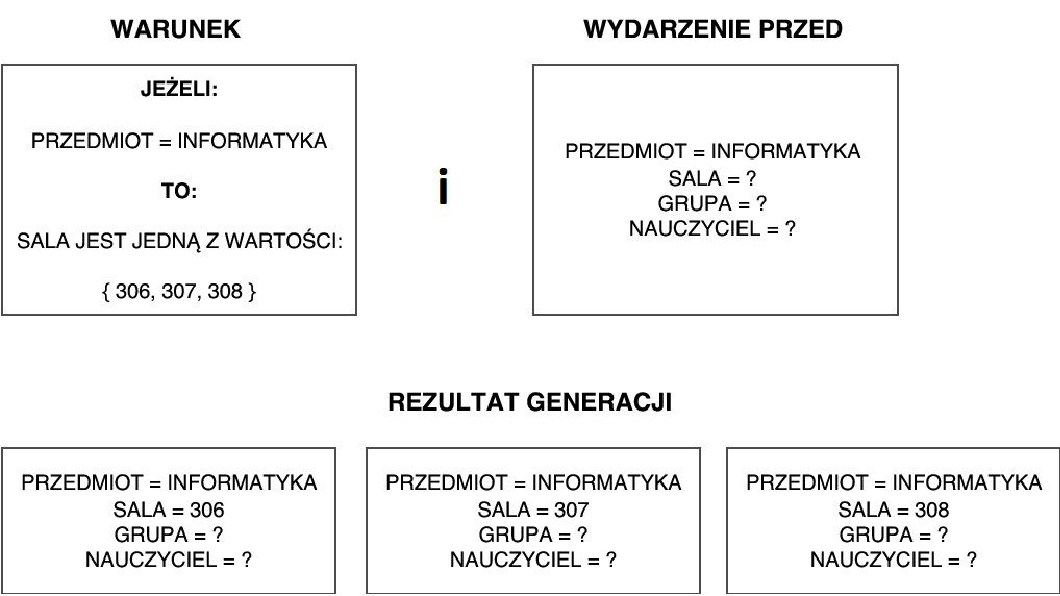
\includegraphics[width=1.0\textwidth]{./img/RezultatGeneracjiLiteraI.pdf}
	\caption{Rezultat generacji dla poprawnego warunku i wydarzenia bazowego}
	\label{id:fig:RezultatGeneracji}
\end{figure}

Nasuwa się pytanie, co jeżeli użytkownik wprowadzi niemożliwe do zrealizowania warunki lub niewystarczające do poprawnej generacji dane? W jaki sposób powinien zachować się program i~sam generator w przypadku gdy ciąg przyczynowo-skutkowy się zapętla i~wymusza inną wartość właściwości, która była źródłem całego ciągu? Podczas analizy wyodrębniono następujące stany uniemożliwiające automatyczne generowanie propozycji dla pojedynczych wydarzeń:
\begin{itemize}
\item niedeterminowalność właściwości --- brak determinantów wypełnionych wartościami właściwości wydarzenia wejściowego, lub brak jakiejkolwiek właściwości o~wartości powiązanej z~jakimkolwiek warunkiem;
\item niezagnieżdżalność wydarzenia --- brak miejsca w~harmonogramie, w~którym można osadzić którykolwiek z~wygenerowanych wydarzeń. Dla rys. \ref{id:fig:RezultatGeneracji} byłaby to sytuacja, gdy sale o numerze 306, 307, 308 mają pełny grafik;
\item kolizja warunków --- istnieje kilka determinantów pewnej właściwości wydarzenia, których oczekiwane wartości nie posiadają części wspólnej. Sytuację taką ilustruje rys. \ref{id:fig:KolizjaWarunkow}. Można na nim zobaczyć, że zbiory oczekiwanych wartości dla numeru sali w~warunkach nie mają części wspólnej, a~wydarzenie bazowe zawiera właściwości, których wartości są powiązane z wyrażeniem warunkowym danych warunków. Dla przykładu z~rys. \ref{id:fig:RezultatGeneracji} miałoby to miejsce, gdyby dodano jeszcze jeden podobny warunek, lecz jego zbiór oczekiwanych wartości nie zawierałby żadnej ze zbioru wartości {306, 307, 308};
\begin{figure}
	\centering
	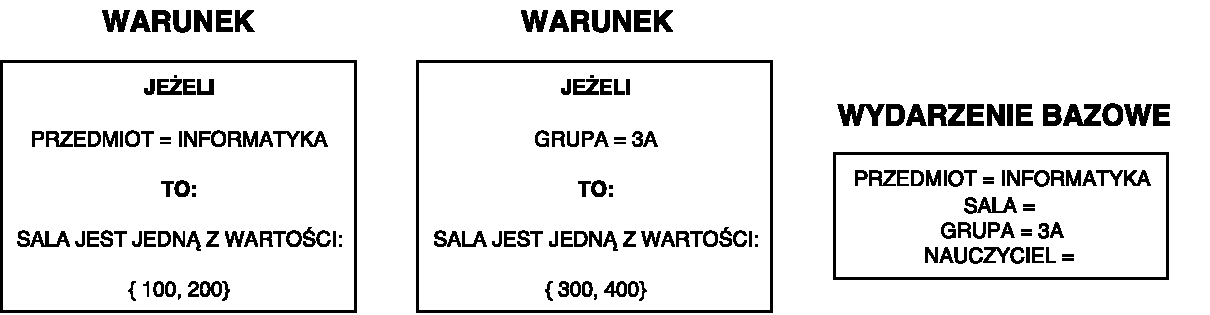
\includegraphics[width=1.0\textwidth]{./img/KolizjaWarunkow.pdf}
	\caption{Kolizja warunków}
	\label{id:fig:KolizjaWarunkow}
\end{figure}
\item niespójność właściwości --- ciąg przyczynowo-skutkowy generacji, lub wartości właściwości w~wejściowym wydarzeniu są niezgodne z warunkami. Występuje w~przypadku, gdy aktualna wartość pewnej właściwości jest sprzeczna z~którymkolwiek z~warunków wpływających na generacje wydarzenia. Jeżeli właściwość \lstinline|Sala| ma wartość \lstinline|305| i~jednocześnie w~tym samym wydarzeniu istnieje inna właściwość \lstinline|Grupa| o~wartości \lstinline|6A|, z~którą powiązany jest warunek determinujący wartość pierwszej wspomnianej właściwości, np. \lstinline|Jeżeli Grupa=6A to Sala=128|, to występuje niespójność właściwości, dlatego że aktualna wartość sali (305) nie pokrywa się z wartością wymuszaną przez warunek. Na rys. \ref{id:fig:Niespojnosc} przedstawiono przykład niespójności przyczynowo-skutkowej, w~której do niespójności dochodzi podczas kolejnych kroków generacji. Zakładając, że wydarzenie bazowe ma właściwość \lstinline|Nauczyciel: Jan Kowalski| to po pierwszym kroku właściwość \lstinline|Sala| przyjmie wartość \lstinline|100| ze względu na warunek \lstinline|Jeżeli Nauczyciel=Jan Kowalski to Sala=100|. W~drugim kroku właściwość \lstinline|Dzień| przyjmie wartość \lstinline|Piątek| i~od tego momentu wydarzenie jest w stanie niespójności, dlatego że jeden z warunków mówi o tym, że jeżeli właściwość \lstinline|Nauczyciel| ma wartość \lstinline|Jan Kowalski| to \lstinline|Dzień| musi być którąś z~wartości \lstinline|{Wtorek, Środa, Czwartek}|. Niespójność spowodowana jest tym, że aktualna wartość dnia to \lstinline|Piątek| i~została ona wygenerowana poprzez inny warunek w~poprzednich krokach generacji.
\end{itemize}
\begin{figure}
	\centering
	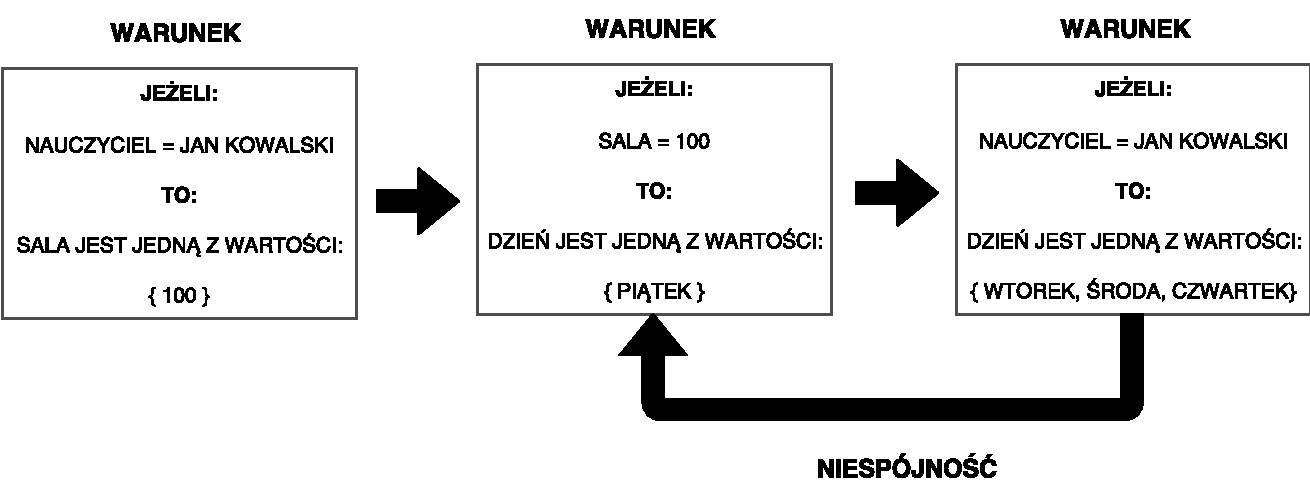
\includegraphics[width=1.0\textwidth]{./img/Niespojnosc.pdf}
	\caption{Niespójność przyczynowo-skutkowa}
	\label{id:fig:Niespojnosc}
\end{figure}

\section{Kryterium wyboru najlepszego zestawu wydarzeń}
\label{wspolczynnikAlg}

W~przypadku gdy algorytm generujący zwróci kilka zestawów właściwości, które spełniają warunki generacji, potrzebny jest sposób na wybranie najlepszego spośród nich. Potrzebny jest zatem pewien współczynnik, którego wartość będzie w~stanie odróżnić poszczególne rozwiązania od siebie i~wskazać najwłaściwsze. Do wyznacznia formuły owego współczynnika wykorzystano podstawowe metody statystyczne takie jak średnia arytmetyczna, odchylenie standardowe, kurtoza. Tabela \ref{tab:alg1} prezentuje dziesięć sześcioelementowych zestawów zajętości właściwości. Liczby przyporządkowane danym właściwościom to ich zajętość. Zajętość mówi o~tym, w~jak wielu wydarzeniach dana właściwość bierze udział, np. zajętość o~wartości 4 dla danego nauczyciela oznacza, że prowadzi on już cztery lekcje. Najbardziej równomierny rozkład zajętości posiadają, w~kolejności od najlepszego, zestawy o~numerach 1, 2, 3 i 9, 10. Spośród nich, najlepszym zdecydowanie jest zestaw nr 1. Zadaniem było wyznaczyć taki współczynnik, który będzie w~stanie uformować ranking o~wspomnianej wcześniej kolejności. Ponadto, ma on brać pod uwagę nie tylko spłaszczenie rozkładu, ale również jego ogólną zajętość. Wyniki obliczeń przedstawia tabela \ref{tab:alg2}. Wybrane miary mają swoje słabe punkty, np. spłaszczenie rozkładu zestawów o~numerach 1 oraz 10 jest takie samo, mają one równe odchylnie standardowe. Ze względu na ogólną zajętość zestawu 10-tego jest on najgorszym z~możliwych wyborów. Samo odchylenie zatem nie wystarczy. Ponadto, średnia będzie zawsze taka sama, jeżeli suma zajętości różnych zestawów jest sobie równa. Nie pozwoli to jednoznacznie odróżnić od siebie danych zestawów. Alternatywą odchylenia standardowego jest wykorzystanie kurtozy. Jest ona miarą spłaszczenia i~koncentracji. Niestety jej wartości są znacznie bardziej problematyczne i~dają gorsze wyniki od odchylenia. Zadowalającym rozwiązaniem okazało się połączenie średniej z~odchyleniem, które niweluje ich słabości, dzięki ich zsumowaniu. Odchylenie dobrze określa rozrzut pomiędzy zajętościami a~dodana do niego średnia pozwala odrzucić zestawy o~podobnym rozrzucie, lecz większej zajętości. Współczynnik obliczany jest według wzoru \ref{id:wspWzor}.
\begin{equation}
\sqrt{\frac{1}{N} \sum_{i=1}^N (x_i - \overline{x})^2} + \overline{x}
\label{id:wspWzor}
\end{equation}

\begin{table}
	\centering
	\caption{Sześcioelementowe zestawy zajętości właściwości}
	\label{tab:alg1}
	\begin{tabular}{cccccccccc}
		\toprule
		\multicolumn{10}{c}{numery zestawów} \\
		1.  & 2. & 3. & 4. & 5. & 6. & 7. & 8. & 9. & 10. \\
		\midrule
		1 & 2 & 3 & 4 & 5 & 6 & 4 & 3 & 2 & 5 \\
		1 & 0 & 0 & 0 & 0 & 0 & 0 & 0 & 0 & 5 \\
		1 & 1 & 0 & 0 & 0 & 0 & 0 & 0 & 0 & 5 \\
		1 & 1 & 1 & 0 & 0 & 0 & 0 & 0 & 0 & 5 \\
		1 & 1 & 1 & 1 & 0 & 0 & 0 & 0 & 2 & 5 \\
		1 & 1 & 1 & 1 & 1 & 0 & 2 & 3 & 2 & 5 \\
		\bottomrule
	\end{tabular}
\end{table}

\begin{table}
	\centering
	\caption{Wyniki obliczeń dla wybranych miar.}
	\label{tab:alg2}
	\begin{tabular}{ccccccccccc}
		\toprule
		\multicolumn{1}{c}{miara} & \multicolumn{10}{c}{numery zestawów}  \\
		& 1.  & 2. & 3. & 4. & 5. & 6. & 7. & 8. & 9. & 10. \\
		\midrule
		średnia          & 1.00 & 1.00 & 1.00 & 1.00 & 1.00 & 1.00 & 1.00 & 1.00 & 1.00 & 5.00 \\
		odch. std. pop.  & 0.00 & 0.57 & 1.00 & 1.41 & 1.82 & 2.23 & 1.52 & 1.41 & 1.00 & 0.00 \\
		kurtoza 		 & - & 2.50 & 2.50 & 3.95 & 5.12 & 6.00 & 1.42 & -1.87 & -3.33 & - \\
		średnia + odch.  & 1 & 1.57 & 2.00 & 2.41 & 2.82 & 3.23 & 2.52 & 2.41 & 2.00 & 5.00 \\
		\bottomrule
	\end{tabular}
\end{table}

\section{Mechanizm generujący harmonogram}
Automatyczne generowanie harmonogramu zaplanowano tak, aby przebiegało w~dwóch etapach. Pierwszym z~nich jest przygotowanie propozycji zestawów właściwości dla każdego wydarzenia bazowego, czyli takiego, którego właściwości są częściowo wypełnione przez użytkownika. Dla każdego wydarzenia bazowego algorytm generujący propozycje powinien znaleźć wszystkie zestawy zgodne z~podanym zbiorem warunków generacji. Po zakończeniu tego etapu możliwe jest odrzucenie części wydarzeń niemożliwych do wygenerowania z~powodu konfliktów lub braku warunków determinujących właściwości bazowe.

Podczas drugiego etapu mechanizm dla każdego wydarzenia grupuje propozycje mu przypisane, korzystając ze współczynnika opisanego w~sekcji \ref{wspolczynnikAlg} tego rozdziału. Zaczynając od najlepszych propozycji, próbuje on wstawić wydarzenie do harmonogramu. Jeżeli ramy czasowe wydarzenia nie są ustalone, mechanizm musi znaleźć w~harmonogramie wolne miejsca. Należy wziąć pod uwagę, że ramy czasowe również są właściwością wydarzenia, więc z~zestawu wolnych miejsc należy wybrać takie, które nie wywołuje niespójności właściwości. Jeżeli nie uda się umieścic zdarzenia w~harmonogramie, mechanizm powinien próbować aż do wyczerpania propozycji. Wynikiem drugiego etapu są umieszczone w~harmonogramie wydarzenia i~raporty o~niepowodzeniach dla każdego wydarzenia, którego generacja się nie powiodła. Realizację mechanizmu można znaleźć w~rozdziale \ref{implMechanizmuGen}.

\section{Manualne tworzenie i edycja harmonogramów}
Podstawową funkcjonalnością systemu powinna być możliwość ręcznego tworzenia i~usuwania wydarzeń w~harmonogramie. Manualne edytowanie planu powinno być możliwe po użyciu automatycznej generacji, przewiduje się bowiem, że automatyczny generator może nie spełnić oczekiwań, lub nie wygenerować pełnego rozwiązania. W~takim wypadku użytkownik powinien mieć możliwość wprowadzania zmian. Podczas takich operacji, aplikacja powinna czuwać zarówno nad spójnością, jak i~zgodnością z~warunkami. Nic nie stoi na przeszkodzie, aby automatycznego generatora nie wykorzystać w~ogóle. Użytkownik dalej może wprowadzać wydarzenia do harmonogramu. Może on wykorzystać warunki jako strażników, aby nie popełnić błędu podczas ręcznego budowania planu lekcji. 

\section{Technologie i narzędzia}
Stworzenie systemu informatycznego wymaga użycia takich technologii i narzędzi, które sprawdzą się w~kontekście celu tworzonej aplikacji. Ma ona wspomagać placówki edukacyjne i~pomagać w~rozwiązaniu skomplikowanego problemu. Ze względu na jego złożoność, oprogramowanie powinno mieć możliwość ciągłego rozwoju w~celu ulepszania zastosowanych heurystyk oraz wprowadzania nowych, które mogą dawać lepsze rezultaty. Ponadto, mając na uwadze potencjalnie duży czas obliczeń w~przypadku zastosowania dokładnych mechanizmów, należy zapewnić możliwość pracy asynchronicznej, a nawet realizacji systemu rozproszonego. Aby zwiększyć atrakcyjność budowanego narzędzia, zdecydowano się na formę aplikacji internetowej, która w~obecnych czasach jest bardzo popularna. Poniższa lista prezentuje zestaw technologii i narzędzi zastosowanych w projekcie:

\begin{itemize}
	\item Java --- język został wybrany głównie z powodu przeważającej wiedzy i doświadczenia autora pracy na temat tego języka, w porównaniu do innych;
	\item Maven \cite{id:Maven} --- narzędzie na platformę Java, służące do automatyzacji budowy oprogramowania. Pozwala w bardzo prosty sposób dołączyć zewnętrzne zależności w postaci bibliotek, wymagając zaledwie podania ich nazwy, paczki, oraz pożądanej wersji, które znajdują się w centralnym repozytorium Mavena \cite{id:MVNrepository}. Plik konfiguracyjny tego narzędzia daje możliwość wygenerowania  pliku zawierającego archiwa ze źródłami programu oraz wszystkich używanych bibliotek, gotowy do tego, by od razu ulokować do na serwerze. Ponadto proces budowania poprzez owo narzędzie składa się z cyklu operacji takich jak walidacja projektu oraz źródeł programu, wykonanie testów jednostkowych i integracyjnych, weryfikacja zbudowanego pliku oraz umieszczenie go w repozytorium lokalnym dzięki czemu paczka może być wykorzystywana jako zewnętrzna biblioteka w innych projektach. Narzędzie wspiera również architekturę mikroserwisów, dzięki możliwości dzielenia projektu na niezależne moduły;
	\item Spring \cite{id:Spring} --- biblioteka ułatwiająca tworzenie oprogramowania, oferująca zestaw przydatnych modułów pozwalających uczynić kod czystszym oraz bardziej rozwijalnym. Wykorzystanie tej biblioteki w rozwijającym się projekcie wspiera jego utrzymanie. Posiada moduł obsługi transakcji, jest kontenerem inwersji kontroli (ang. \ang{Inversion of Control}, IOC) pozwalającym na efektywne zastosowanie wzorca wstrzykiwania zależności (ang. \ang{Dependency Injection}, DI). Zawiera również moduł dostępu do danych, który pozwala na integrację z biblioteką Hibernate, oraz moduł wspierający wzorzec Model-Widok-Kontroler (ang. \ang{Model-View-Controller}, MVC), za pomocą którego w nieskomplikowany sposób można udostępnić zewnętrzny interfejs komunikacyjny oparty o serwis REST;
	\item Vaadin \cite{id:Vaadin} --- platforma deweloperska zawierająca komponenty przeznaczone do tworzenia przeglądarkowego interfejsu użytkownika w stylu aplikacji jednostronowej (ang. \ang{Single-page application}, SPA). Daje możliwość budowania interfejsu użytkownika z poziomu kodu, bez wymagania znajomości i użycia innych języków takich jak HTML czy JavaScript. Dzięki temu osoba biegła w języku Java jest w stanie pracować nad warstwą logiki biznesowej jak i interfejsu użytkownika, jak również ich wzajemnej interakcji. Nie neguje to jednak wykorzystania innych technologii przez osoby w nich biegłe, ponieważ udostępnia narzędzia pozwalające dostosowanie interfejsu do potrzeb użytkownika, poprzez możliwość edycji kaskadowych arkuszów stylów (ang. \ang{Cascading Style Sheets}, CSS), oraz wstawiania skryptów JavaScript;
	\item Apache Tomcat \cite{id:ApacheTomcat} --- serwer będący kontenerem javowych serwletów, nie posiada pełnego zakresu funkcjonalności serwerów aplikacji Javy Korporacyjnej (ang. \ang{Java Enterprise Edition}, JEE), jednakże w zupełności sprawdza się jako serwer aplikacji internetowych wykorzystujących bibliotekę Spring. Jako, że zastosowane narzędzie Vaadin wykorzystuje serwlety, serwer ten zdaje się być odpowiednim wyborem;
	\item PostgreSQL \cite{id:PostgreSQL} i pgAdmin \cite{id:pgAdmin} --- baza danych została wybrana głównie z powodu braku większego doświadczenia autora z innymi bazami. Dedykowane oprogramowanie pgAdmin do zarządzania bazą jest niezwykle proste w obsłudze i uruchomienie takiej bazy przebiega szybko i bezproblemowo. Ponadto jest to produkt darmowy;
	\item Hibernate \cite{id:Hibernate} --- biblioteka realizująca warstwę dostępu do danych zgodna z oficjalnym standardem mapowania obiektowo-relacyjnego dla języka Java. Jest ona najpopularniejszym rozwiązaniem oraz jest integrowalna z wykorzystaną biblioteką Spring. Pozwala na mapowanie za pomocą javowych adnotacji i może zainicjalizować bazę danych podczas startu aplikacji, przez co nie jest konieczne użycie odpowiednich skryptów SQL.
	\item RabbitMQ \cite{id:RabbitMQ} --- oprogramowanie pośredniczące przeznaczone do kolejkowania i przekierowywania komunikatów. Pełni funkcję nadzorcy i dyspozytora wiadomości. Zastosowanie tego narzędzia jest krokiem ku dalszemu rozwojowi aplikacji. Integracja z nim otwiera możliwości odciążenia wątku głównego aplikacji, poprzez delegację złożonych obliczeniowo, lub blokujących interfejs użytkownika, procedur do niezależnych wykonawców. Pozwala w nieskomplikowany sposób zwiększyć stopień rozproszenia systemu.
\end{itemize}


\chapter{Wymagania funkcjonalne i niefunkcjonalne}
%\begin{itemize}
%\item wymagania funkcjonalne i~niefunkcjonalne
%\item przypadki użycia (diagramy UML)
%\end{itemize}

Na podstawie analizy oraz zdefiniowania problemu ustalono cel realizacji projektu oraz założenia, które ma on spełniać. Zakres funkcjonalności, które dostarczyć ma tworzone oprogramowanie przedstawia następująca lista wymagań:

\begin{itemize}
	\item narzędzie będzie aplikacją przeglądarkową;
	\item każda szkoła będzie posiadała własnego administratora;
	\item administrator szkoły będzie mógł dodawać użytkowników o~różnych uprawnieniach;
	\item nauczyciele będą mieli dostęp tylko do odczytu;
	\item aplikacja umożliwi wprowadzanie do systemu nauczycieli, sale, grupy uczniów oraz listę przedmiotów szkolnych;
	\item będzie można wprowadzać kilku nauczycieli na raz w~jednym okienku, tyczy się to również sal i~grup;
	\item użytkownik będzie miał możliwość ręcznego tworzenia planu lekcji poprzez samodzielne dodawanie wydarzeń do planu lekcji;
	\item wydarzenia będzie można dodawać bezpośrednio z~poziomu widoku planu lekcji, klikając w~odpowiednie pole na harmonogramie;
	\item wprowadzane wydarzenia nie będą musiały być kompletne. Część ich właściwości będzie mogła zostać pusta i~zostanie oznaczona pytajnikiem.
	\item aplikacja umożliwi sprawdzanie poprawności wydarzenia przed jego wstawieniem do planu, informując użytkownika o~występujących konfliktach;
	\item plan lekcji będzie można wyświetlać w~kontekście konkretnego nauczyciela, sali oraz grupy;
	\item narzędzie umożliwi automatyczne wygenerowanie planu na podstawie ustalonych przez użytkownika warunków;
	\item warunki będą wprowadzane do systemu przez użytkownika i~będą zapisywane, nie będzie konieczności wpisywania warunków przy każdym wykorzystywaniu automatycznej generacji;
	\item automatyczny generator będzie wypełniał puste właściwości w~wydarzeniach, których właściwości są częściowo wypełnione (wydarzenia bazowe);
	\item aplikacja umożliwi dodanie tego samego wydarzenia kilkakrotnie w~jednym okienku, poprzez wpisanie liczby kopii;
	\item status i~konflikty, które wystąpiły podczas automatycznej generacji będzie można zobaczyć na osobnym panelu.
\end{itemize}
Oprócz wymagań co do zakresu funkcji systemu, zdefiniowano kilka technicznych założeń, które projektowany system ma realizować. Są one następujące:
\begin{itemize}
	\item narzędzie ma być zaprojektowane w~oparciu o~techniki i~koncepcje projektowania sterowanego dziedziną;
	\item oprogramowanie ma realizować architurę wielotenantową;
	\item oprogramowanie ma wykorzystywać architekturę sterowaną zdarzeniami
	\item narzędzie ma być zintegrowane z~oprogramowaniem pośredniczącym do przesyłania komunikatów.
\end{itemize}



\chapter{Specyfikacja zewnętrzna}

%\begin{itemize}
%\item wymagania sprzętowe i~programowe
%\item sposób instalacji
%\item sposób aktywacji
%\item instalacja
%\item kategorie użytkowników
%\item sposób obsługi
%\item administracja systemem
%\item kwestie bezpieczeństwa
%\item przykład działania, scenariusze korzystania z~systemu, ilustrowane zrzutami z~ekranu lub generowanymi dokumentami
%\end{itemize}
Tworzona aplikacja jest oparta o~aktualne technologie informatyczne. Jest to aplikacja działająca na platformie Java w~64-bitowym środowisku maszyny wirtualnej Javy (ang. \ang{Java Virtual Machine}, JVM). Oprogramowanie jest niezależne od systemu operacyjnego. Graficzny interfejs użytkownika jest przystosowany głównie do przeglądarki Google Chrome. Program pracuje w~oparciu o bazę danych PostgreSQL. Do uruchomienia programu wymagane są następujące narzędzia, w~nawiasach podano ich wspierane wersje, działanie na innych nie było testowane.

\begin{itemize}
	\item serwer Apache Tomcat (8.0.43);
	\item serwer z bazą danych PostgreSQL (9.5) oraz narzędzie do jego administracji (pgAdmin III);
	\item serwer oprogramowania RabbitMQ (3.6.9);
	\item przeglądarka internetowa (Google Chrome);
\end{itemize}

\section{Standardowa instalacja}
Instrukcja ta obejmuje podstawową instalację systemu lokalnie na maszynie pracującej na systemie operacyjnym Windows 10, przy użyciu wymaganych narzędzi w~zalecanych wersjach. Potrzebne są skompilowane źródła programu w~postaci pliku \lstinline|scheduler-webapp-1.0-SNAPSHOT.war|, dostępne na dołączonej płycie CD. Wymagane narzędzia należy zainstalować

\section{Zaawansowana instalacja}

\section{Użytkownicy i administracja systemem}
Aplikacja posiada trzy role użytkowników oraz jednego unikalnego superużytkownika, którym jest administrator całego systemu. Poszczególne role użytkowników to:
\begin{itemize}
	\item administrator tenanta --- nie posiada ograniczeń co do użycia funkcjonalności aplikacji. Jako jedyny może dodawać innych użytkowników i~nimi zarządzać. Wszyscy użytkownicy utworzeni przez danego administratora tenanta mają dostęp do tego samego zasobu danych (patrz \ref{architekturaMultitenant});
	\item dyrekcja --- ma dostęp do wszystkich funkcjonalności aplikacji oprócz zarządzania użytkownikami;
	\item nauczyciel --- posiada uprawnienia jedynie do odczytu, nie może wprowadzać żadnych danych do systemu.
\end{itemize}
Rolą superadministratora jest dodawanie nowych administratorów tenantów. Taki lokalny administrator może tworzyć innych użytkowników o~takiej samej roli, ale wciąż w~ramach tego samego tenanta. Aby zalogować się do panelu superadministratora, należy otworzyć stronę o~adresie serwera z~końcówką ,,\lstinline|/internalPanel|''. Standardowe dane do logowania superadministratora to:
{\renewcommand\labelitemi{}
\begin{itemize}
	\item login: \lstinline|admin@a.pl|
	\item hasło: \lstinline|admin1|
\end{itemize}
Aby zmienić te dane należy wykonać zaawansowaną instalację systemu. Widok logowania oraz dodawania nowego administratora przedstawiono na rys. \ref{id:fig:superAdmin}.
\begin{figure}
	\centering
	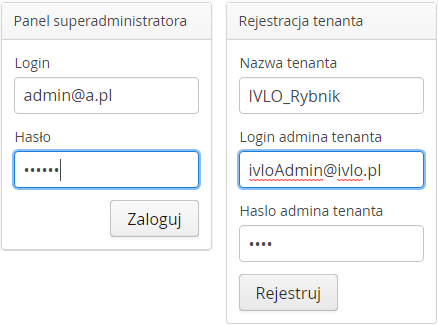
\includegraphics[ height=0.22\textheight]{./img/superAdmin.png}
	\caption{Panel superadministratora}
	\label{id:fig:superAdmin}
\end{figure}
Z~poziomu konta administratora tenanta możliwe jest dodawanie nowych użytkowników. W~prawym górnym rogu ekranu widnieje komponent oznaczony nazwą \lstinline|Konto|, jak przedstawia rys. \ref{id:fig:newUser}. Po jego zaznaczeniu rozwija się lista, w~której znajduje się opcja \lstinline|Uzytkownicy|. Należy ją wybrać aby przejść do widoku dodawania nowych użytkowników.
\begin{figure}
	\centering
	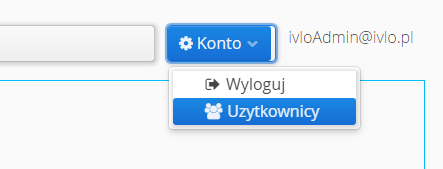
\includegraphics[ height=0.15\textheight]{./img/newUser.png}
	\caption{Przejście do panelu dodawania nowych użytkowników}
	\label{id:fig:newUser}
\end{figure}
Widok użytkowników składa się z tabeli o~dwóch kolumnach, kolejno nazwie użytkownika oraz jego roli. Po prawej stronie tabeli znajduje się panel z~przyciskami, za pomocą którego można dodawać i~usuwać nowych użytkowników, oraz odświeżać tabelę. Po wybraniu opcji \lstinline|Dodaj| wyświetla się okno w~które należy wpisać odpowiednie dane oraz wybrać rolę użytkownika. Panel z~przyciskami oraz okno dodawania użytkownika ilustruje rys. \ref{id:fig:newUser2}. Po zakończeniu dodawania należy kliknąć przycisk \lstinline|Odśwież|. Mogą wystąpić pewne opóźnienia w~wykonywaniu operacji. Aby usunąc użytkownika, należy zaznaczyć go w~tabeli oraz kliknąc przycisk \lstinline|Usuń|. Tylko użytkownicy o~roli administratora tenanta mają uprawnienia do zarządzania użytkownikami.
\begin{figure}
	\centering
	\includegraphics[ height=0.25\textheight]{./img/newUser2.png}
	\caption{Dodawanie nowego użytkownika.}
	\label{id:fig:newUser2}
\end{figure}

\section{Logowanie i główny widok aplikacji}
Ekran logowania dostępny jest pod adresem serwera z~końcówką \lstinline|/app|. Po wybraniu takiego adresu z~poziomu przeglądarki powinien ukazać się widok z~panelem logowania. Aby wylogować się z systemu, należy nacisnąć komponent \lstinline|Konto| znajdujący się w~górnym prawym rogu i~wybrać opcję \lstinline|Wyloguj|. Wspomniany komponent widnieje na rys. \ref{id:fig:newUser}.

Aplikacja składa się z~dwóch kluczowych komponentów. Są to pasek narzędzi widniejący w~górnej części widoku oraz panel główny aplikacji zajmujący większość ekranu. Pasek narzędzi prezentuje się tak jak na ilustracji \ref{id:fig:toolbar}. Panel początkowo jest pusty, dopiero po wybraniu opcji z~paska narzędzi zmienia on swój stan, przechodząc do odpowiedniego widoku.
\begin{figure}
	\centering
	
\includegraphics[width=1.0\textwidth]{./img/toolbar.png}
	\caption{Pasek narzędzi.}
	\label{id:fig:toolbar}
\end{figure}
\section{Dodawanie nauczycieli, sal, grup i przedmiotów}
Wszystkie podmioty wspomniane w~tytule mają podobny widok. Składa się on z~tabeli zajmującej większą część ekranu oraz kilku przycisków pozwalających zarządzać danym podmiotem. Ponadto, widok dodawania każdego z~opisywanych podmiotów jest możliwe kilkakrotnie w~jednym oknie. Służy temu przycisk \lstinline|Dodaj następny|. Do okna dodawana jest wtedy kolejna pusta pozycja, pozwalająca dodać kolejny element. Kilkukrotne dodawanie danego podmiotu przedstawiono na rys. \ref{id:fig:multiAdd}. Podmiotem dodawanym jest nauczyciel.
\begin{figure}
	\centering
	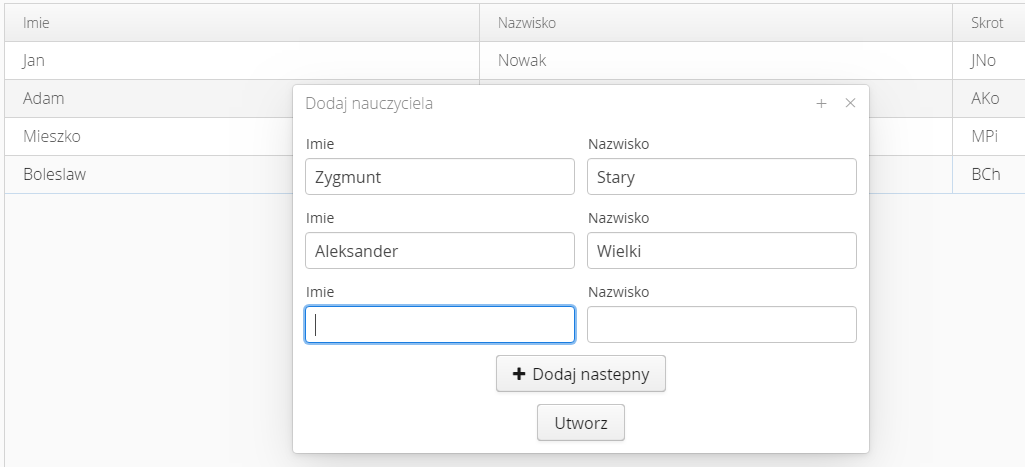
\includegraphics[width=1.0\textwidth]{./img/multiAdd.png}
	\caption{Wielokrotne dodawanie nauczycieli w~jednym oknie.}
	\label{id:fig:multiAdd}
\end{figure}

\section{Definiowanie warunków generacji}
Widok warunków składa się z~dwóch tabel. Jedna z~nich jest osadzona w~paneliu wraz z~przyciskami zarządzania. Tabela składa się z~dwóch kolumn, kolejno właściwość warunkowa i~właściwość wymuszana, jej fragment przedstawiono na rys. \ref{id:fig:warunki1}. Właściwość warunkowa mówi o~tym, że w~przypadku wystąpienia takiego podmiotu w~wydarzeniu, inna właściwość musi przyjąć jedną z~wartości wymuszanych. Jaka to będzie wartość i~której właściwości będzie dotyczyć definiowana jest właśnie przez właściwość wymuszaną. Druga kolumna jednak pokazuje jedynie jej nazwę, a~nie zestaw wartości, które ta właściwość może przybrać. Służy do tego druga tabela, umieszczona po prawej stronie widoku. Po kliknięciu w~dany wiersz w~pierwszej tabeli, druga automatycznie uzupełnia się o~odpowiednie wartości. Można ją zobaczyć na wspomnianym rysunku, prezentuje ona wartości wymuszane dla właściwości o nazwie \lstinline|dzień|.
\begin{figure}
	\centering
	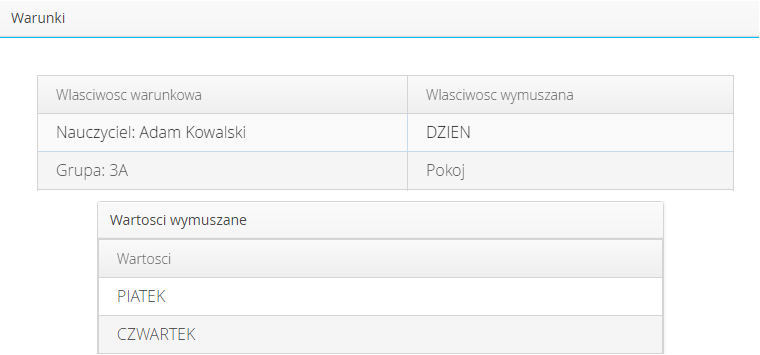
\includegraphics[width=1.0\textwidth]{./img/warunki1.png}
	\caption{Tabele panelu warunków generacji.}
	\label{id:fig:warunki1}
\end{figure}

\section{Tworzenie wydarzeń bazowych i automatyczne generowanie}
Wydarzenia bazowe, czyli takie, które posiada tylko część wypełnionych właściwości, tworzy się w~panelu dostępnym pod menu rozwijanym z~elementu o~nazwie \lstinline|Plany| paska narzędzi, wybierając opcję \lstinline|Zdarzenia|. Wyświetla się wtedy widok niemal identyczny jak w~przypadku warunków generacji. Jedyne różnice to zawartość panelu zarządzania, który zawiera znacznie więcej opcji. W~oknie dodawania takiego wydarzenia, jak przedstawia rys. \ref{id:fig:wydBazowe1}, pola można wypełniać jedynie wybierając opcje z~listy rozwijanej. Znajdują się na niej tylko takie podmioty, które zdefiniowano w~systemie. Istnieje również możliwość utworzenia kilku wydarzeń bazowych w~jednym okienku. Należy w~odpowiednie pole tekstowe wpisać liczbę wydarzeń, które mają być utworzone. Dzięki temu w~łatwy sposób można wprowadzić do systemu np. wszystkie informatyki dla pewnej grupy. Automatyczny generator dobierze godziny samemu.
\begin{figure}
	\centering
	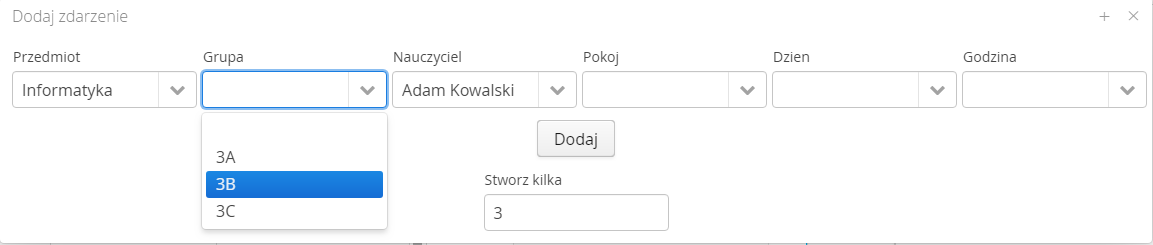
\includegraphics[width=1.0\textwidth]{./img/wydBazowe.png}
	\caption{Okno dodawania wydarzenia bazowego.}
	\label{id:fig:wydBazowe1}
\end{figure}

Sam widok składa się z~dwóch tabel. Po lewej stronie wyświetlane są informacje o~wydarzeniu, a~klikając w~odpowiedni wiersz, tabela po prawej wyświetli wszystkie właściwości danego wydarzenia, jak ilustruje rys. \ref{id:fig:wydBazowe2}. Mając już zdefiniowany zbiór wydarzeń bazowych, wystarczy kliknąć przycisk \lstinline|Generuj harmonogram|. Wydarzenia mają swoje statusy. Początkowo przyjmują one status \lstinline|NOWY|, czyli taki, który został dopiero utworzony i~nie został poddany generacji i~nie jest osadzony w~harmonogramie. Po generacji status może zmienić się na jeden z przedstawionej listy:
\begin{itemize}
	\item kolizja --- podczas generacji wystąpił konflikt typu niespójność właściwości lub kolizja warunków;
	\item niedeterminowalny --- nie ma podstaw do wyznaczenia którejkolwiek z~właściwości wydarzenia;
	\item zagnieżdżony --- wygenerowano poprawną propozycję oraz udało osadzić się wydarzenie w~planie;
	\item niezagnieżdżalny --- nie udało się osadzić wydarzenia w~planie. Powodem może być ogólny brak miejsc w~planie lub brak takich miejsc, które nie powodują konfliktów w~propozycjach generowanych wydarzeń.
\end{itemize}
Jeżeli podczas generacji wystąpił konflikt, wydarzenie o~takim statusie można zaznaczyć w~tabeli i~zobaczyć raport o~niepowodzeniach, zawierający ich przyczynę oraz obiekt konfliktu. Aby wyświetlić te informacje, należy po zaznaczeniu wydarzenia kliknąć w~przycisk \lstinline|Pokaż niespójności| lub \lstinline|Pokaż kolizje|. Są to dwa różne typy konfliktów, które zostały opisane w~rozdziale \ref{sterowanieiproblemy}. Informacje o~nich wyświetlane sa w~odrębnych oknach.
\begin{figure}
	\centering
	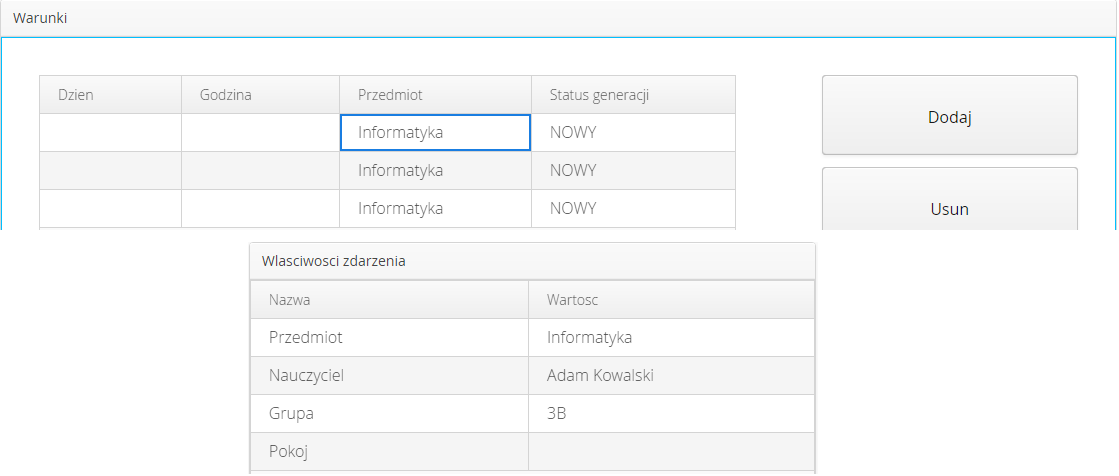
\includegraphics[width=1.0\textwidth]{./img/wydBazowe2.png}
	\caption{Przykładowe wydarznenia bazowe i ich właściwości.}
	\label{id:fig:wydBazowe2}
\end{figure}




\section{Podgląd i manualna edycja planu lekcji}
Bieżący plan lekcji można podejrzeć poprzez wybranie opcji \lstinline|Aktualny plan| z~elementu o nazwie \lstinline|Plany| na pasku narzędzi. Wyświetla się wtedy pusty plan, dlatego że wpierw należy wybrać podmiot względem którego owy plan będzie przedstawiony. Należy to zrobić wykorzystując komponent rozwijanej listy znajdujący się po prawej stronie planu lekcji, oznaczony napisem \lstinline|Plan dla|. Nie można pokazać planu lekcji dla przedmiotów, jedyne opcje to podmioty takie jak nauczyciele, grupy, sale. Każdy taki podmiot, który jest wprowadzony do systemu ma swój plan. Fragment widoku planu lekcji przedstawia rys. \ref{id:fig:fragmentPlan}.
\begin{figure}
	\centering
	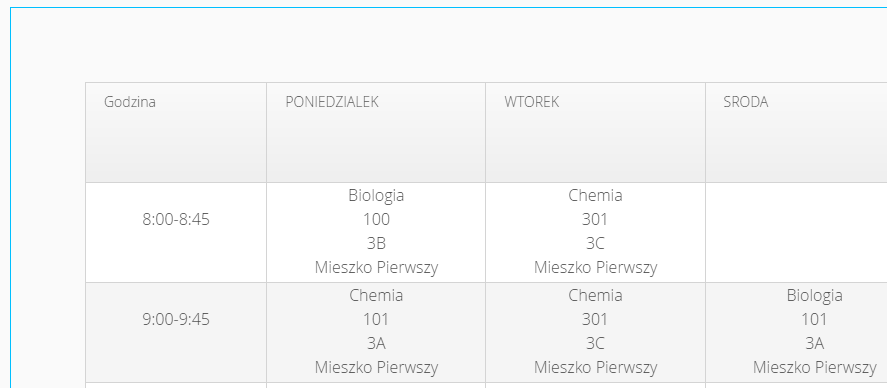
\includegraphics[width=1.0\textwidth]{./img/fragmentPlan.png}
	\caption{Fragment widoku planu lekcji.}
	\label{id:fig:fragmentPlan}
\end{figure}
Z~panelu planu lekcji możliwe jest bezpośrednie dodanie do niego wydarzenia. Kliknięcie w~dowolne pole pozwala na edycję wydarzenia, jeżeli takie się tam znajduje, lub dodanie nowego. Podczas dodawania wydarzenia dostępna jest opcja sprawdzenia poprawności wydarzenia pod względem konfliktów takich jak niespójność właściwości i~kolizja warunków. Jeżeli takowe zaistnieją, na ekranie wyświetli się okno z~raportem niepowodzeń. Dodatkowo, sprawdzana jest dostępność każdego podmiotu partycypującego w~aktualnie wprowadzanym wydarzeniu. Jeżeli dany podmiot jest już zajęty w~danym czasie, na ekranie pojawi się informacja o~konflikcie miejsc. Okno dodawania wydarzenia i~edycji wygląda tak jak na rys. \ref{id:fig:dodawanieDoPlanu}.
\begin{figure}
	\centering
	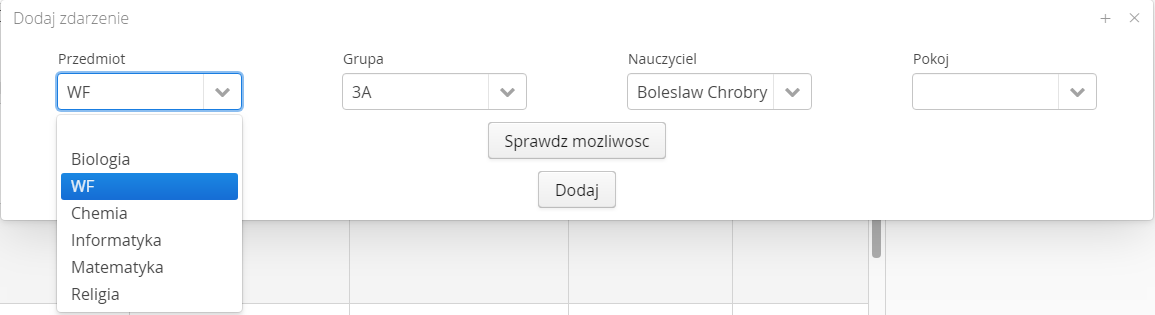
\includegraphics[width=1.0\textwidth]{./img/dodawanieDoPlanu.png}
	\caption{Okno dodawania i edycji wydarzenia z poziomu planu lekcji.}
	\label{id:fig:dodawanieDoPlanu}
\end{figure}

\chapter{Specyfikacja wewnętrzna}
%\begin{itemize}
%\item przedstawienie idei
%\item architektura systemu
%\item organizacja baz danych
%\item komponenty, moduły, biblioteki
%\item przegląd ważniejszych klas
%\item przegląd ważniejszych algorytmów
%\item szczegóły implementacji wybranych fragmentów
%\item diagramy UML
%\end{itemize}



\section{Architektura systemu}
%\addtocontents{toc}{\setcounter{tocdepth}{3}}


Architektura, wg standardu ISO/IEC/IEEE 42010-20110, to ,,zasadnicze koncepcje lub właściwości systemu w jego środowisku, zawarte w jego elementach, relacjach i w zasadach jego projektowania i ewolucji'' \cite{id:ieee2011_Architecture}.Według tego standardu, architektura powinna posiadać pewne cechy dotyczące nie tylko formy elementów budujących system, ale i zależności między tymi elementami. Powinna opisywać sposób, w~jaki forma i~relacje między jej elementami zapewniają działanie systemu. Architektura składa się z zestawu charakterystycznych dla danego systemu zasad wskazujących sposób, w~jaki powinien być implementowany~i rozszerzany system w konkretnych jego obszarach. Nie ma ograniczeń co do tego, co może być elementem systemu. Może to być nawet inny system, posiadający swoją architekturę.

Mówiąc o architekturze nie sposób nie natknąć się na pojęcie takie jak ,,system''. Podobnie jak architektura, definicji systemu można znaleźć kilka. Według standardu IEEE Std 1471-2000 \cite{id:ieee2000_Architecture} brzmi ona:
\begin{quote}
	,,Zestaw komponentów zorganizowanych, tak by pełnić pewną funkcję lub zestaw funkcji.''
\end{quote}
Wynika z tego, że systemem może być praktycznie wszystko, co zbudowane jest z elementów współpracujących ze sobą w ramach zestawu i dostarcza określoną funkcjonalność. Zatem nie jest nieprawidłowym stwierdzenie, że aplikacja jest systemem.

Niniejszy rozdział skupia się na opisie ważniejszych obszarów tworzonej aplikacji, koncepcji, zasad działania, oraz stosowanych wzorców. Wyjaśnia ona sposób korzystania z elementów architektury, objaśnia sens ich stosowania, oraz traktuje o tym jak powinien zachowywać się system w specyficznych dla kontekstu elementów architektury sytuacjach.

\subsection{Architektura sterowana zdarzeniami (EDA)}
Architektura sterowana zdarzeniami (ang. \ang{Event Driven Architecture}, EDA) jest wzorcem architektonicznym zgodnym z paradygmatem programowania sterowanego zdarzeniami (programowane zdarzeniowe). Opiera się na generowaniu i~przesyłaniu zdarzeń, reagowaniu na nie bądź ich ignorowaniu. Zdarzeniami są konkretne sytuacje występujące w programie. Model zdarzenia nie jest ściśle określony, można go jednak podzielić na dwie części, takie jak nagłówek i ciało. Nagłówek składa się z informacji o wystąpieniu zdarzenia i pozwala na jego rozpoznanie, zawiera takie informacje, jak typ czy identyfikator, ciało natomiast powinno zawierać wszystkie potrzebne odbiorcy informacje opisujące to zdarzenie \cite{id:EDA_BrendaMichelson}. Charakterystyczną cechą EDA jest możliwość wybierania przez odbiorców tylko tych zdarzeń, o których zaistnieniu chcą być informowani, oraz możliwość wysyłania zdarzeń do wielu odbiorców na raz \cite{id:maximeKlusman}. Takie podejście jest zgodnie ze wzorcem publikuj-subskrybuj (ang. \ang{publish-subscribe}), który cechuje się skalowalnością, co pośrednio przenosi się na omawianą architekturę.

Implementacje EDA zazwyczaj korzystają z asynchroniczności. Wersja synchroniczna niestety nie przynosi dużych korzyści. Są to jedynie takie udoskonalenia jak standaryzacja kodu, możliwość łatwej implementacji wzorca segregacji odpowiedzialności komend i zapytań (ang. \ang{Command Query Responsibility Segregation}, CQRS) (którego struktura jest prawie taka sama jak struktura EDA), bądź wspomaganie wzorca pozyskiwania zdarzeń (ang. \ang{Event Sourcing}, ES). W dużych aplikacjach, szczególnie webowych i wieloużytkownikowych czy takich które działają po stronie serwera, a nie klienta, ważna jest wydajność. Kolejkowanie zdarzeń i wykonywanie ich asynchronicznie zwalnia źródło zdarzenia z konieczności czekania na jego zakończenie \cite{id:hohpe2006programming,id:maximeKlusman}. Jako architektura, EDA definiuje nie tylko pewien rodzaj struktury, ale również sposób zachowania \cite{id:ibm_Architecture}, który zakłada używanie zdarzeń w kluczowych dla dziedziny momentach. Dziedzinę rozumie się jako pewną sferę wiedzy, obszar tematyczny oprogramowania, obszar zainteresowania użytkownika \cite{id:sobotka_SDJ-DDD,id:DDD_Evans}. Przykładem może być program księgowy, którego dziedziną są pieniądze i finanse. Ważnym zdarzeniem w kontekście dziedziny takiego programu może być utworzenie faktury i każda zmiana z nią związana, taka jak przykładowo jej wystawienie, czy opłacenie przez klienta. Stosowanie takiego podejścia skutkuje automatycznym tworzeniem ścieżki audytu, co wspiera ES.

Pożądanymi cechami, które charakteryzują opisywaną architekturę są luźne powiązania (ang. \ang{loose coupling}) oraz duże rozproszenie \cite{id:EDA_BrendaMichelson}. Obie te cechy wzajemnie się uzupełniają. W systemie luźno powiązanym, tworzące go komponenty posiadają niewielką wiedzę o innych. Powinny być one na tyle niezależne od siebie, aby zmiany jednym z nich, nie pociągały za sobą konieczności zmian w innych komponentach, z nim powiązanych. W EDA źródło zdarzenia, publikując je, nie ma pojęcia o jego odbiorcach, jaka będzie reakcja na owo zdarzenie, ani w jaki sposób informacja o zdarzeniu dotrze do odbiorcy.  Luźne powiązania osiągane są często przez użycie popularnego wzorca wstrzykiwania zależności (ang. Dependency Injection, DI), co jest zgodne z dobrą praktyką tworzenia oprogramowania obiektowego zwaną zasadą pojedynczej odpowiedzialności (ang. \ang{Single Responsibility Principle}, SRP). EDA jest często budowana w oparciu o oprogramowanie pośredniczące zorientowane na komunikaty (ang. \ang{Message-Oriented Middleware}, MOM). Podejście takie wspiera asynchroniczność oraz równoważenie obciążenia, bowiem przetwarzanie pewnych zdarzeń może być realizowane przez dedykowane temu aplikacje zainstalowane na odrębnych serwerach. Użycie takiego oprogramowania nawet w aplikacji, która nie jest fizycznie rozproszona, ma pewne zalety. Zazwyczaj takie oprogramowanie jest dobrze zoptymalizowane oraz wspiera często stosowane rozwiązania.


\subsubsection{Paradygmat programowania zdarzeniowego}

Struktura omawianej architektury wcale nie pozwala jednoznacznie określić jej przeznaczenia. Jak wspomniano w opisie, architektura ta jest zgodna z paradygmatem  programowania sterowanego zdarzeniami. ,,Programowanie zdarzeniowe (inaczej: sterowane zdarzeniami) to takie, gdy program składa się z wielu niezależnych podprogramów, których kolejność wykonania nie jest określona z góry przez program główny, lecz które są uruchamiane w reakcji na zaistnienie pewnych zdarzeń'' \cite{id:bylina}. Definicja ta mówi jednej z cech programu, który realizuje ten paradygmat. Chodzi o brak możliwości ustalenia momentu wywołania danego bloku programu, który jest reakcją na zaistnienie sytuacji niemożliwej do zdeterminowania na podstawie ciągu instrukcji programu. Program bowiem nie zawiera informacji pozwalających przykładowo na ustalenie momentu wciśnięcia przycisku przez użytkownika. Programista natomiast może spodziewać się wystąpienia takich sytuacji. Pojęcie \emph{zdarzenie} nie jest ściśle określone. Może być określone jako znacząca zmiana stanu systemu \cite{id:EDA_GartnerSummit} lub coś wymagającego uwagi, co występuje w aplikacji lub poza nią \cite{id:EDA_BrendaMichelson}. W programowaniu zazwyczaj zdarzenie odnosi się do konkretnej sytuacji i wynikających z niej konsekwencji, wobec których wystąpienia podejmuje się akcję. Bardzo ważną cechą zdarzenia jest fakt, że z punktu widzenia działania programu zdarzenie jest na tyle istotne, że wydziela się dla niego fragment mający za zadanie podjąć akcję w momencie jego zaistnienia.


\subsubsection{Struktura architektury sterowanej zdarzeniami}



EDA dzieli się na minimum trzy warstwy:

\begin{itemize}
	\item Warstwa generująca obejmuje miejsca, gdzie jest przygotowywany i tworzony podmiot reprezentujący zdarzenie, który następnie jest publikowany do warstwy komunikacji. Generatorem może być dowolny element systemu, zarówno z warstwy oprogramowania jak i sprzętowej.
	\item Warstwa komunikacji zapewnia, by wygenerowane zdarzenie zostało odebrane przez zainteresowane nim komponenty. Warstwa ta zazwyczaj składa się z kolejki, w której przetrzymywane są zdarzenia, elementy przekazujące (ang. \ang{dispatcher, router}), których zadaniem jest dostarczenie odbiorcom informacji o zaistniałym zdarzeniu, w przyjętej w danym środowisku formie.
	\item Warstwa przetwarzająca, do której należą elementy systemu, które są informowane o wystąpieniu zdarzenia i zazwyczaj podejmują pewne akcje w odpowiedzi na jego zaistnienie. W tej warstwie może zostać wygenerowane i opublikowane inne zdarzenie, jednakże jego źródłem dalej pozostaje najwcześniej opublikowane zdarzenie. Zwykle zawiera elementy nasłuchujące (ang. \ang{listener}) i obsługujące (ang. \ang{handler}).
\end{itemize}

Stopień złożoności tych warstw jest bardzo różny, im bardziej rozszerza się strukturę, tym większe może przynieść korzyści. EDA cechuje się dużym rozproszeniem, a każdą jej warstwę można implementować na wiele sposobów, otrzymując pożądane efekty. Ograniczać ją pod względem technicznym może tylko środowisko, w którym powstaje. Każda z warstw może znajdować się w odrębnym środowisku, ze względu na obecność warstwy komunikacyjnej, która je ze sobą łączy.

\begin{figure}
	\centering
	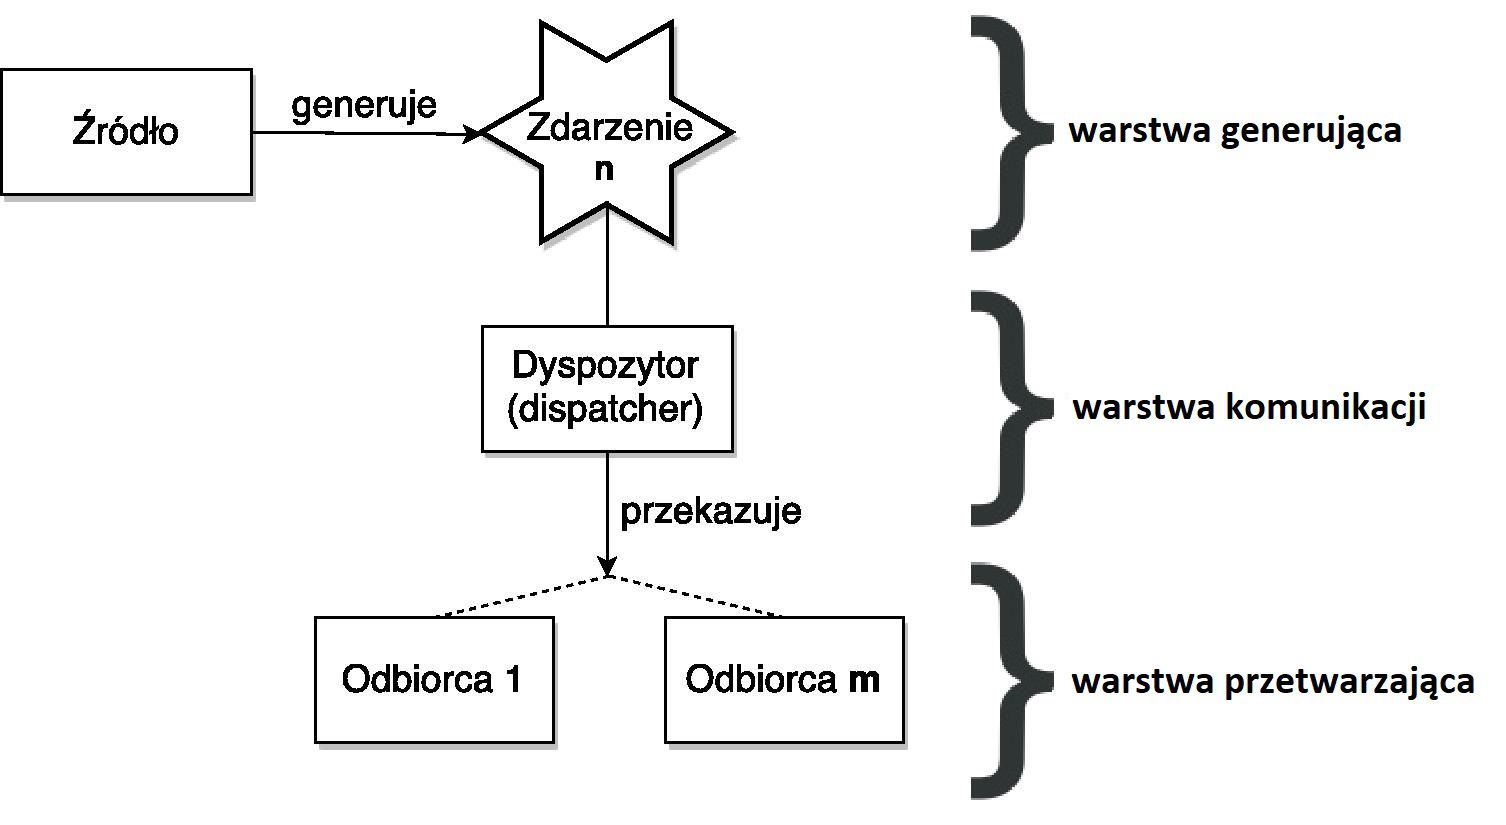
\includegraphics[width=1.0\textwidth]{./img/EDA_GeneralSchema.pdf}
	\caption{Podstawowa struktura EDA.}
	\label{id:fig:1}
\end{figure}

Na rysunku \ref{id:fig:1} przedstawiono prosty schemat struktury EDA, podzielonej na wspomniane warstwy. Ilustracja zawiera pewne nieokreślone źródło, generujące dowolne zdarzenie. Jest ono następnie przekazane do dyspozytora, którego zadaniem jest dostarczenie wiadomości do wszystkich zainteresowanych nią odbiorców. Dyspozytora można zatem porównać do listonosza, a nawet placówki pocztowej. Jego ważną cechą jest to, że po przejęciu opublikowanego zdarzenia jest on za nie odpowiedzialny. Opublikowane zdarzenie powinno przebywać w warstwie komunikacji tak długo, aż zostanie przetworzone przez odbiorcę, jeżeli takowy istnieje. Zdarzenie nie powinno wracać do źródła, wynika to z~założen EDA, które traktują o~tym, że źródło nie jest zainteresowane dalszymi losami zdarzenia.


Naturalny przepływ programu nie korzystającego z wielowątkowości może powodować blokadę źródła, co jest niezgodne z koncepcją EDA, bowiem zakłada ona, że źródło zdarzenia nie czeka na obsługę. Implementacja synchroniczna oparta o~omawianą ilustrację nie zapewni tej cechy. Źródło przedstawione na rys. \ref{id:fig:2}, przekazując zdarzenie do dyspozytora, musi wywołać jego metodę. Jeżeli metoda ta nie działa w~osobnym wątku, źródło będzie zmuszone czekać na jej zakończnie. To samo tyczy się dyspozytora, który będzie zablokowany na czas obsługi zdarzenia, jeżeli elementy obsługujące również nie pracują w osobnym wątku. Rys. \ref{id:fig:listingEDA1} przedstawia kod programu, który działa zgodnie z~opisaną sytuacją. Podczas pracy programu, w metodzie \lstinline|foo()|, po opublikowaniu zdarzenia, metoda \lstinline|continueFoo()| dojdzie do skutku dopiero po zakończeniu metody \lstinline|dispatch()|, ta natomiast zostanie odblokowana po przetworzeniu zdarzenia przez odbiorców. Struktura EDA nie jest skomplikowana, problematyczne jednakże mogą być konkretne wymagania funkcjonalne projektowanego systemu, które mogą znacznie zwiększać stopień skomplikowania implementacji.
\begin{figure}
	\centering
	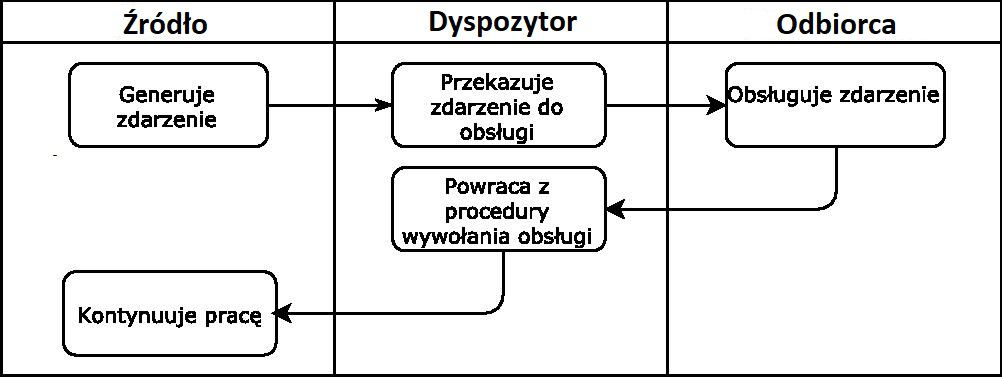
\includegraphics[width=1.0\textwidth]{./img/EDA_FlowSynchro.pdf}
	\caption{Naturalny przepływ programu na podstawie rysunku \ref{id:fig:1}}
	\label{id:fig:2}
\end{figure}
\begin{figure} 
\begin{lstlisting}
public void foo() {
	bar();
	publisher.publish(new FooEvent());
	continueFoo();
}

public void publish(Event e) {
	dispatcher.dispatch(e);
}

public void dispatch(Event e) {
	handlers.foreach(handler -> {
		if(handler.isInterestedIn(e)) {
			handler.handle(e);
		}
	});
}
\end{lstlisting}
\caption{Fragment synchronicznego przepływu programu implementującego EDA}
\label{id:fig:listingEDA1}
\end{figure}

Elementem, którego nie da się ominąć mówiąc o podejściu sterowanym zdarzeniami, jest forma zdarzenia, inaczej model. Jego reprezentacja jest dowolna, jednakże musi być zawierać pewnego rodzaju informacje. Dane pozwalające zidentyfikować zdarzenie to jego nagłówek. Drugą częścią jest ciało, które zawiera niezbędne dane, pozwalające na przetworzenie zdarzenia. W przypadku nagłówka można z góry określić jego strukturę. Ciało natomiast powinno być możliwe do modelowania na dowolny, lub zgodny z określonym standardem sposób, ponieważ zdarzenia mogą nie być ze sobą w żaden sposób powiązanie dziedzinowo, przez co mogą być opisywane na całkiem różne sposoby. Obiekt zdarzenia powinien być niezmienny (ang. \ang{immutable}), czyli niemożliwy do modyfikacji.

\subsubsection{Rozmaitość implementacji i rozwiązania problemów EDA}

Wygodnym rozwiązaniem problemu zależności czasowych pomiędzy warstwą generującą a pozostałymi, jest podzielenie struktury na dwa wątki --- główny aplikacji, oraz obsługi zdarzeń. Takie rozwiązanie ilustruje rysunek \ref{id:fig:3}. Wątek obsługi zdarzeń powinien obejmować warstwę komunikacyjną oraz przetwarzającą. Źródło generujące zdarzenie przekazuje je dyspozytorowi, który jest odseparowany od wątku głównego aplikacji, dzięki czemu przetwarzanie ma miejsce równolegle. Wywołanie metody pewnego obiektu skutkuje jej uruchomieniem w ramach tego samego wątku, w którym jest wywoływana. Metody dyspozytora zatem muszą być wywoływane przez wątek, w~którym się znajduje. Najprostszym sposobem by uzyskać taką funkcjonalność, jest uruchomienie dyspozytora w nieskończonej pętli, która będzie cały czas oczekiwała na przyjęcie zdarzenia. Te z kolei należy składować w pewnym obszarze dostępnym z poziomu dyspozytora. Użyteczna do tego zadania jest kolejka. Główna metoda dyspozytora nieprzerwanie odpytuje kolejkę w celu pobrania elementów tam składowanych. Wątek główny aplikacji, chcąc wywołać obsługę zdarzenia, powinien opublikować je we wspomnianej kolejce. Opisane rozwiązanie przedstawia listing na rys. \ref{id:fig:listing:dispatcher}.

\begin{figure}
\begin{lstlisting}
public class Dispatcher extends Thread {
	private Queue<Event> queue;
	
	public void run() {
		while(true) {
			if(queue.notEmpty()) {
				dispatch(queue.poll());
			}
		}
	}
}
\end{lstlisting}
\caption{Dyspozytor z kolejką}
\label{id:fig:listing:dispatcher}
\end{figure}

\begin{figure}
	\centering
	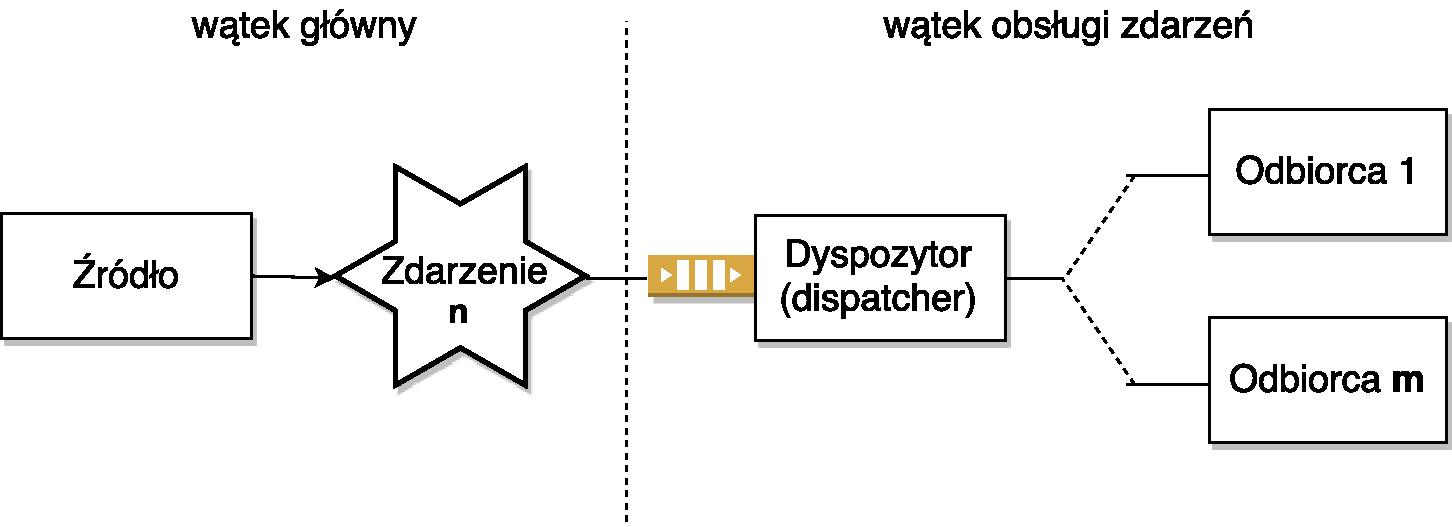
\includegraphics[width=1.0\textwidth]{./img/EDA_AsyncDispatcher.pdf}
	\caption{Struktura zapewniająca brak powiązań czasowych, z podziałem na dwa wątki.}
	\label{id:fig:3}
\end{figure}

Rażącą nieoptymalnością tego rozwiązania jest aktywne czekanie (ang. \ang{busy waiting, polling}). Polega ono na ciągłym sprawdzaniu pewnego warunku czy też odpytywaniu o stan obiektu, oczekując na zielone światło w celu wykonania operacji. W przypadku listingu na rys. \ref{id:fig:listing:dispatcher}, program w nieskończonej pętli sprawdza, czy istnieje w kolejce zdarzenie. Każde przejście pętli marnuje cykle procesora, które mogą być wykorzystane przez inne procesy. Rozwiązaniem jest użycie monitorów, czyli mechanizmu blokowania pewnego wątku, dopóki inny go nie odblokuje. Java posiada swoją implementację monitorów w formie procedur \lstinline|wait()| i \lstinline|notify()|. Wywołanie metody \lstinline|wait()| powoduje zatrzymanie wątku do czasu otrzymania sygnału z innego wątku, który następuje przez wywołanie metody \lstinline|notify()|. Zablokowanie ciągle działającego, aczkolwiek nie wykonującego jakichkolwiek konkretnych operacji wątku, można zrealizować w sposób przedstawiony na rys. \ref{id:fig:listing:dispatcherWithoutBusyWaiting}. Listing ten przedstawia wątek działający w nieskończonej pętli, ciągle powtarzający procedurę \lstinline|process()|. Po każdym jej uruchomieniu sprawdzane jest, czy kolejka zawiera zdarzenia do przetworzenia. Jeżeli tak, zdarzenie jest z niej pobierane oraz przekazane do odbiorców. W przeciwnym wypadku wątek zostaje zatrzymany, nie marnując cykli procesora poprzez aktywne czekanie. Odblokować go może tylko inny wątek, który wykona metodę \lstinline|addEventToQueue()|. Po opublikowaniu zdarzenia w kolejce, wątek działający w nieskończonej pętli zostaje odblokowany w celu dalszego działania.

\begin{figure}
\begin{lstlisting}
	public void run() {
		while(true) {
			process();
		}
	}
	
	private void process() {
		if(queue.isEmpty()) {
			wait();
		}
		dispatch(queue.poll());
	}
	
	private void addEventToQueue(Event e) {
		queue.add(e);
		notify();
	}
}
\end{lstlisting}
\caption{Działanie dyspozytora w osobnym wątku, niewrażliwe na aktywne czekanie}
\label{id:fig:listing:dispatcherWithoutBusyWaiting}
\end{figure}
Rozwiązanie problemu przez podział na aplikacji na dwa wątki nie jest jedynym sposobem implementacji zapewniającej potrzebne funkcjonalności. W przypadku dużego rozproszenia systemu, wielu odbiorców zdarzeń czy znacznego obciążenia systemu przez generowane zdarzenia, przedstawiona na rysunku \ref{id:fig:4} struktura może być wydajniejsza. W odróżnieniu od poprzednio opisywanego podejścia, kolejka nie stanowi już części dyspozytora. Jest ona umieszczona w każdym z obslugiwaczy. Ponadto, pracują one w osobnych wątkach. Dzięki zastosowanej strategii, sam dyspozytor może działać w wątku głównym aplikacji, ponieważ identyfikacja i przesłanie zdarzenia do odpowiednich odbiorców nie powinny być złożone czasowo. Pewną wadą tego rozwiązania jest jednak zdjęcie odpowiedzialności dyspozytora, którą jest dopilnowanie aby zdarzenie zostało przetworzone prawidłowo. Łatwiej jest takową dostarczyć, gdy całość procesu nadzoruje jeden obiekt. Gdy wspomniana funkcjonalność jest wymagana, dobrym rozwiązaniem jest zaprojektowanie odbiorców i dyspozytora tak, by komunikowały się między sobą w celu potwierdzenia przetworzenia żądania. Stosując tę strategię należy z rozwagą dysponować ilością wątków. Dobrą praktyką może być ograniczenie jej puli i rozdzielanie ich pomiędzy kilku odbiorców.

\begin{figure}
	\centering
	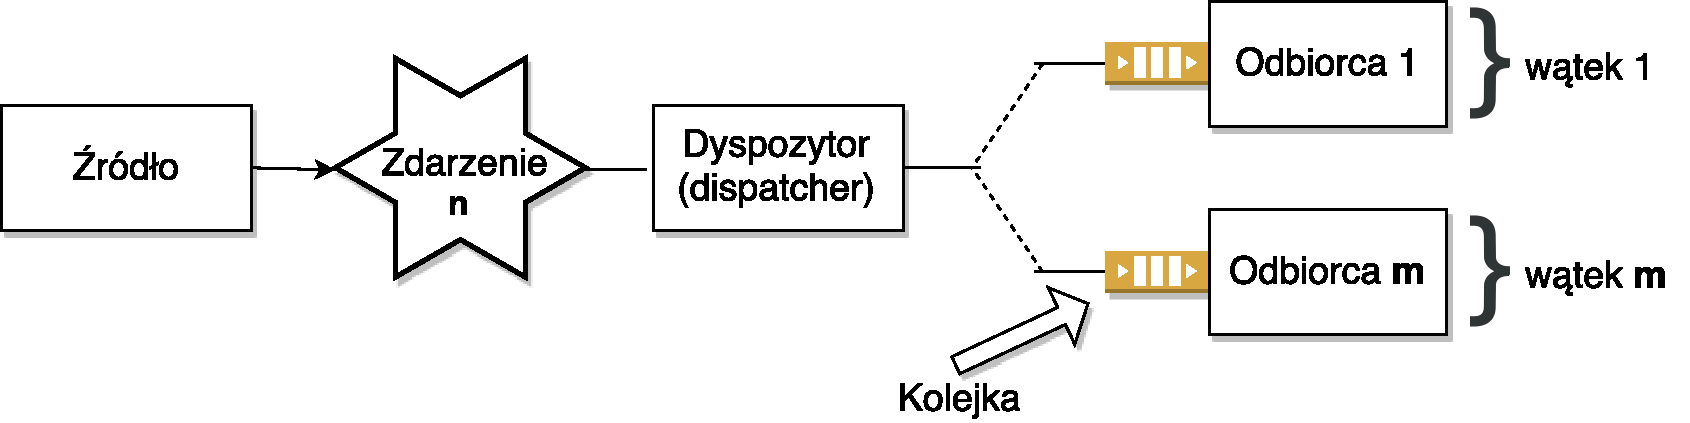
\includegraphics[width=1.0\textwidth]{./img/EDA_AsyncHandler.pdf}
	\caption{Struktura zapewniająca brak powiązań czasowych, z podziałem na dwa wątki.}
	\label{id:fig:4}
\end{figure}

\subsubsection{Oprogramowanie pośredniczące zorientowane na komunikaty (MOM)}
Kluczowym dla systemów o znacznym rozproszeniu w kontekście oprogramowania jak i sprzętu, jest warstwa komunikacyjna. Ważną częścią pracy poszczególnych modułów aplikacji jest komunikacja między nimi. W EDA za te zadania odpowiada głównie dyspozytor. Należy go wyposażyć w mechanizmy zapewniające pożądaną pracę wspomnianej warstwy systemu. Sytuacja ulega skomplikowaniu, gdy wymagana jest transakcyjność, składowanie obiektów zdarzeń na dysku, czy zgodność z pewnym protokołem komunikacyjnym. Dochodzą do tego równie ważne kwestie, opisane w poprzednich częściach rozdziału. Mowa tutaj o zjawisku pollingu, potrzebie kolejkowania, potwierdzania wykonania obsługi, podziału na wątki. Oprogramowanie pośredniczące zorientowane na komunikaty (ang. \ang{Message-Oriented Middleware}, MOM) należy właśnie do warstwy komunikacyjnej. Może zapewniać wszystkie poruszane wcześniej kwestie. Ponadto, może posiadać zoptymalizowane algorytmy dostarczania wiadomości i wiele sposobów konfiguracji całej sieci komunikacyjnej przy pomocy wygodnego interfejsu. 

Wykorzystanym MOM w tworzonej aplikacji jest oprogramowanie RabbitMQ \cite{id:RabbitMQ}. RabbitMQ jest rozbudowanym narzędziem służącym do kolejkowania wiadomości i odpowiedzialnym za dostarczanie wiadomości do odbiorców. Zawiera konsolowy jak i również graficzny interfejs przeznaczony do administrowania usługą. Jest systemem oferującym dużą niezawodność, udostępnia funkcje składowania wiadomości na dysku i odtwarzania ich po awarii. Zapewnia transakcyjną komunikację z konsumentami, wymagając potwierdzenia (ACK) pomyślnego przetworzenia wiadomości. Narzędzie to opiera się na kolejkach, konfigurowanych na różne sposoby, do których podłączani są konsumenci.  Oprócz nich, istnieje możliwość zdefiniowania punktu wymian (ang. \ang{exchange}), który pełni funkcję dyspozytora, bowiem dostarcza do odpowiednich kolejek dane wiadomości, jest on wymagany w przypadku korzystania z mnogiej ilości kolejek. Punkt wymian udostępnia kilka sposobów przekazywania wiadomości do kolejek. Wiadomość jak i wiązanie między kolejką a punktem wymian są oznaczone pewnym kluczem lub zestawem atrybutów o konkretnej wartości. Wiadomość trafi do tych kolejek, których oznaczenia wiązań pasują do klucza czy atrybutów (w zależności od konfiguracji). RabbitMQ oferuje następujące tryby pracy punktów wymian:
\begin{itemize}
	\item tryb bezpośredni (ang. \ang{direct exchange}) --- wiadomość trafi do każdej kolejki, której powiązanie ma taki sam klucz jak klucz wiadomości;
	\item tryb wzorcowy (ang. \ang{topic exchange}) --- wiadomość trafi do każdej kolejki powiązanej przy użyciu wzoru, do którego pasuje klucz wiadomości;
	\item tryb atrybutowy (ang. \ang{headers exchange}) --- wiadomość trafi do każdej kolejki powiązanej atrybutami, których wartości są takie same jak wartości atrybutów wiadomości lub są akceptowalne przez kolejkę;
	\item tryb rozgłoszeniowy (ang. \ang{fanout exchange}) --- wiadomość trafi do wszystkich kolejek.
\end{itemize}
\begin{figure}
	\centering
	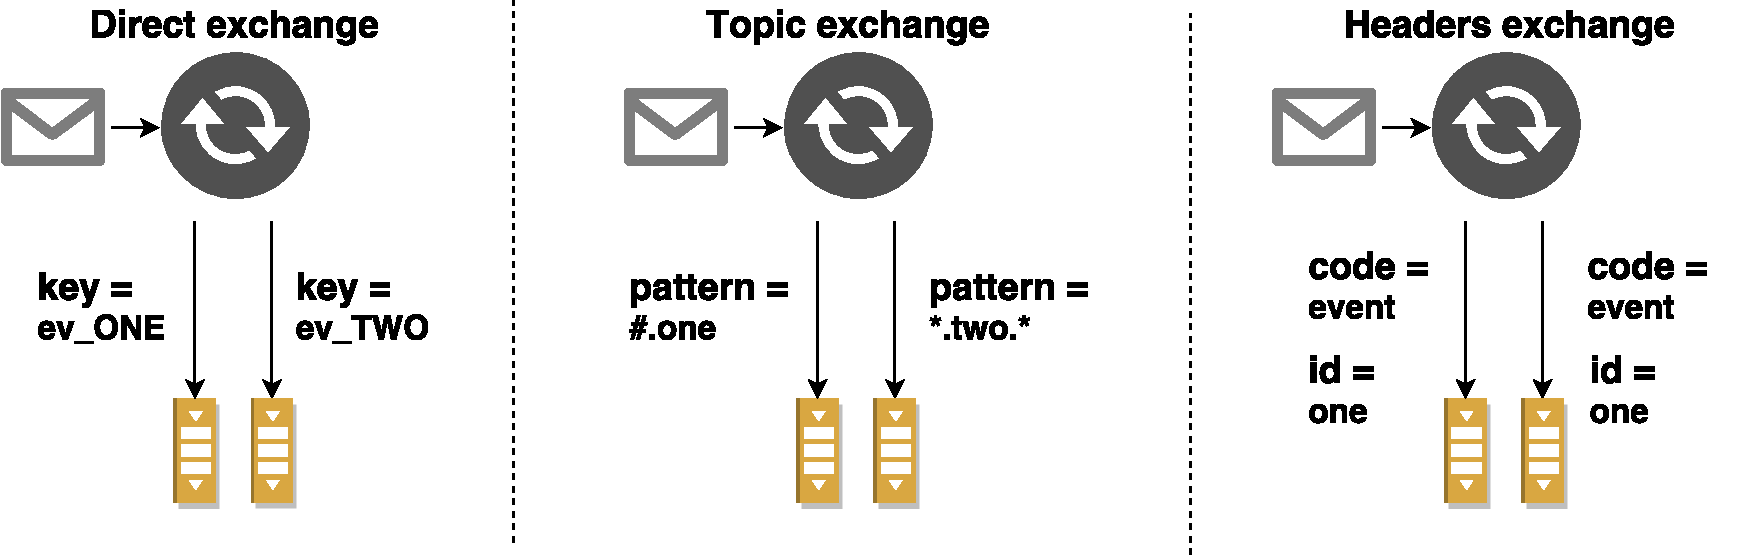
\includegraphics[width=1.0\textwidth]{./img/EDA_Kolejki.pdf}
	\caption{Tryby pracy punktów wymian.}
	\label{id:fig:5}
\end{figure}
%TODO na rysunku id=one jest dwa razy zamiast id=two w drugim przypadku
Na rysunku \ref{id:fig:5} zaprezentowano przykładowe powiązania kolejek z punktami wymian. Rozważmy następujące scenariusze. Opublikowano wiadomość o kluczu \lstinline|ev_ONE| do punktu pracującego w trybie \lstinline|direct|. Taka wiadomość trafi do każdej kolejki, która powiązana jest z tym punktem dokładnie takim kluczem. W przypadku trybu \lstinline|topic| sytuacja nieco się komplikuje. Znak ,,\#'' oznacza dowolny ciąg znaków, a ,,*'' dokładnie jedno słowo. Słowa są oddzielone od siebie kropką. Wiadomość o kluczu \lstinline|any.thing.one| trafi do pierwszej kolejki. Do drugiej może trafić wiadomość o~trójwyrazowym wzorze, takim jak przykładowo \lstinline|any.two.thing|. Kolejnym trybem jest tryb \lstinline|headers|. Posiada on dodatkowy atrybut \lstinline|x-match|, który przyjmuje wartości \lstinline|all| lub \lstinline|any|. W przypadku wybrania opcji \lstinline|all|, wszystkie atrybuty muszą się zgadzać. Wiadomość identyfikująca się jako ,,code = event, id = anything'' nie trafi do żadnej kolejki, dla wartości ,,x-match = any'', wystarczy jeden pasujący atrybut. W takim wypadku wspomniana wiadomość trafi do obu kolejek.


\subsection{Projektowanie sterowane dziedziną (DDD)}
\label{architekturaDDD}

Projektowanie sterowane dziedziną (ang. \ang{Domain-Driven Design}, DDD) to zestaw koncepcji i technik przeznaczonych do projektowania i~implementacji modeli biznesowych \cite{id:sobotka_DDD1}. Jedną z~jego cech jest modyfikacja klasycznej architektury warstwowej. Polega ona na oddzieleniu logiki aplikacji od logiki biznesowej, dzięki temu logika biznesowa jest skupiona jedynie wokół modelu i~jest niezależna od platformy. Każda z warstw zależy jedynie od warstw położonych niżej. Izolują one odpowiedzialności oraz ułatwiają interpretację systemu. Opis poszczególnych warstw przedstawiono na poniższej liście, w~kolejności warstwy najwyższej do najniższej:

\begin{itemize}
	\item warstwa interfejsów --- udostępnia metody sterowania aplikacją oraz dostępu do wyników działań systemu. Może stanowić zarówno graficzny interfejs użytkownika, czy taki oparty o~serwis REST. Warstwa często utożsamiana z~warstwą prezentacji. 
	\item warstwa aplikacji --- spaja całą aplikację w~działający program, wykorzystując wszystkie pozostałe warstwy. Definiuje działania, które wykonuje program i~steruje obiektami dziedzinowymi w~celu rozwiązania postawionych przed nimi zadań. Warstwa ta nie zawiera reguł ani wiedzy biznesowej, jedynie deleguje zadania do warstw niżej. Jej elementy są pewnego rodzaju kontrolerami. W~jej skład wchodzą głównie serwisy aplikacyjne oraz nasłuchiwacze (odbiorcy) zdarzeń.
	\item warstwa dziedziny --- najważniejszą warstwą z~punktu widzenia projektowania sterowanego dziedziną. Zawiera ona strukturę wszystkich elementów systemu oraz logikę biznesową zebraną w~odpowiednich elementach tej warstwy. Reprezentuje reguły jak i~zagadnienia biznesowe. Należą do niej agregaty, encje, obiekty-wartości, interfejsy repozytoriów, serwisy domenowe, definicje zdarzeń;
	\item warstwa infrastruktury --- wspomaga warstwy wyższe poprzez udostępnianie dostępu do elementów i~zasobów z~poza aplikacji. Zawiera implementacje repozytoriów.  
\end{itemize}

DDD definiuje pewien zestaw elementów służących modelowaniu systemu zwanych cegiełkami (ang. \ang{Building Blocks}) \cite{id:sobotka_SDJ-DDD}. Część z~nich została wymieniona jako elementy zawierające się w~warstwach opisanych wcześniej. Dalsza część rozdziału opisuje te elementy, które zostały użyte w~projektowanym systemie.

\subsubsection{Encja (ang. \ang{Entity})}

Encje (ang. \ang{entity}) są obiektami, które nie są bezpośrednio zdefiniowane przez swoje atrybuty, a~przez posiadanie pewnej tożsamości \cite{id:DDD_Evans}. Encja posiada pewną ciągłość życia i~jest odróżnialna na podstawie pewnego unikalnego identyfikatora. Jest pojęciem takim samym jak to, które są znane z~modelowania struktury bazy danych. Przypuszczamy, że może istnieć dwóch nauczycieli o~takim samym imieniu jak i~nazwisku. Nie oznacza to, że są to dwa te same byty. Encje ulegają zmianom na przestrzeni czasu, a~ich właściwości nie identyfikują ich tożsamości. Tym właśnie różnią się od zwykłych obiektów, że posiadają pewną tożsamość. Ponadto, klasy reprezentujące encje wcale nie muszą być pozbawione logiki biznesowej i~stanowić zwykłą strukturę przechowującą dane \cite{id:sobotka_SDJ-DDD}. Niemniej jednak powinny zawierać tylko niezbędną i~wpływającą na stan obiektu logikę.

\subsubsection{Obiekt-wartość}
W~odróżnieniu od encji, obiekt-wartość (ang. \ang{Value Object}, VO) nie posiada żadnej tożsamości. Może on opisywać jedynie pewną charakterystykę rzeczy \cite{id:DDD_Evans}. Dowolny taki obiekt można zastąpić innym o~tych samych atrybutach. Przykładem może być banknot o~pewnej wartości. Mając banknot o~pewnym nominale, możemy go zamienić na inny o~takiej samej wartości. To, czy dane pojęcie klasyfikuje się jako encja lub obiekt-wartość zależy tylko od kontekstu. Z~punktu widzenia aplikacji bankowej rozróżniającej fałszywe banknoty, może być ważny numer seryjny. Pozwala pewnym bytom nadać sens dzięki zgrupowaniu atrybutów pod jedną nazwą. Bardziej klarownym bowiem jest użycie klasy \lstinline|Money|, niżli korzystanie z~typu \lstinline|double|. Ponadto obiekt-wartość również może posiadać pewną logikę, pomagającą w~ich budowaniu jak i~przetwarzaniu.

\subsubsection{Agregaty i korzenie agregatów}
Agregaty to obiekty nadzorujące zestaw danych głównie w~postaci encji i~obiektów-wartości. Agregat tworzy pewnego rodzaju drzewo, ponieważ jedna z~encji go tworzących musi być encją główną, czyli korzeniem (ang. \ang{Aggregate Root}). Zewnętrzne obiekty, chcąc odwołać się do składników agregatu, muszą robić to pośrednio przez sam agregat. Struktura taka zapewnia dużą hermetyzację obiektu. Model obiektowy samochodu byłby agregatem korzeniem zawierającym takie encje jak np. silnik czy bak. Chcąc zatankować samochód należy wykonać to poprzez metody agregatu jakim jest samochód. Nie należy wyciągać baku na zewnątrz samochodu. To logika agregatu, bądź jego serwisu (który jest omówiony w~dalszej części rozdziału) ma umożliwiać takie operacje. Usuwając agregat, usuwamy również kaskadowo wszystkie jego elementy. Są one głównymi obiektami dziedzinowymi w~modelu systemu, ponieważ encje na ogół są zbyt ziarniste i~wykonywanie operacji na każdej z~osobna może skutkować zbyt dużym chaosem. Łącząc kilka powiązanych ze sobą dziedzinowo obiektów w~jeden, system staje się bardziej zrozumiały. 

\subsubsection{Repozytorium}
W~najprostszym ujęciu są to elementy zapewniające dostęp do danych. Repozytoria powinny być tworzone głównie dla agregatów, udostępniając metody do ich składowania i~pobierania na podstawie ich identyfikatorów. Nie powinno zawierać wielu specyficznych metod wyszukujących dane na potrzeby interfejsu użytkownika. Mają one służyć do wprowadzania zmian w~encjach. Powinny zwracać jedynie kopie elementów, nie dając możliwości zmiany stanu encji. Taka zmiana powinna być zatwierdzana dopiero przez repozytorium, odwołując się do elementu poprzez jego identyfikator.

\subsubsection{Serwis domenowy}
Encje mogą posiadać w~sobie logikę biznesową. Jednakże aby nie obciążyć jej zbyt duża odpowiedzialnością, należy pozostawiać jej tylko kluczowe w~cyklu życia encji metody. Istnieją również takie operacje, które nie pasują do encji, np. operacje na całych kolekcjach. Większość logiki zatem powinna znaleźć się w~serwisie domenowym. Służą one tylko pojedynczemu obiektowi domenowemu, zazwyczaj encji, czasami wartości. Może natomiast posiłkować się innymi obiektami domenowymi. Serwisy muszą być one bezstanowe, mają jedynie wykonywać operacje na rzecz obiektów domenowych.

\subsubsection{Serwis aplikacyjny}
Spaja logikę poszczególnych obszarów dziedziny, używając do tego kilku serwisów domenowych. Steruje nimi tak, aby wykonać poszczególne przypadki użycia aplikacji. Przykładem może być encja koszyka oraz produktu w~oprogramowaniu sklepu internetowego. Serwis aplikacyjny posiadając dostęp do serwisów domenowych obu encji może pobrać obiekt produktu z~repozytorium, obliczyć odpowiedni rabat przy użyciu serwisu koszyka oraz dodać do niego produkt. Następnie zatwierdzić zmiany przez zapis do repozotorium.

\subsubsection{Zdarzenie}
Jeżeli pewne działania po zmianie stanu obiektu domenowego muszą wywołać reakcję w~niezależnym obszarze systemu, przydatne są zdarzenia. Przykładem może być wysłanie wiadomości mailowej w~reakcji na zakup przedmiotu. Zdarzenia mogą również służyć obsludze złożonych operacji, bowiem odbiorcy zdarzeń zazwyczaj pracują w~innym wątku. Występują również sytuacje, kiedy chcemy rozluźnić powiązania pomiędzy obiektami. Generujemy wtedy zdarzenie, na które nasłuchiwać mogą odbiorcy z~kilku obszarów dziedziny systemu i~każde z~nich zareaguje wtedy we własnym zakresie. 

\subsection{Wielotenantowość}
\label{architekturaMultitenant}

Oprogramowanie wielotenantowe to takie, którego architektura zaprojektowana jest tak, aby użytkownicy w ramach pewnej grupy dzielili pewien zasób. Wielotenantowość występuje tylko w aplikacjach wieloużytkownikowych.
Tenantem nazywamy grupę użytkowników traktowaną jako jeden podmiot, dzielącą dane, konfigurację czy dostęp do podobnych funkcjonalności, mając wzgląd na prywatność poszczególnych użytkowników \cite{id:Multitenancy}. Na rys. \ref{id:fig:Multitenancy} przedstawiono porównanie zwykłego systemu z takim, który wykorzystuje omawiane zagadnienie. Biorąc jako przykład bibliotekę posiadająca własny system, gdzie użytkownicy to bibliotekarze zgrupowani w ramach tenanta, możemy powiedzieć, że każdy z bibliotekarzy ma dostęp do tych samych książek, informacji o dacie wypożyczenia i tym podobnych danych. Osoba zwracająca książkę wcale nie musi zwracać jej bibliotekarzowi, który wypożyczył jej tę książkę. Bibliotekarz jest częścią tenanta, dzięki czemu może mieć dostęp do danych o tej książce i przyjąć ją spowrotem, jeżeli implementacja systemu na to zezwala. Należy bowiem pamiętać o tym, że dostęp do wspólnych danych i ich edycja w poszczególnych przypadkach jest zależna jedynie od implementacji systemu, tak jak i stopień prywatności użytkowników. W systemie finansowym, główna księgowa może mieć dostęp do faktur przypisanych do wszystkich oddziałów firmy, a młodsze księgowe tylko w ramach oddziału nad którym sprawują pieczę. Zarówno główna księgowa jak i młodsze tworzą jednego tenanta. Jeżeli jedna z księgowych wystawi fakturę, to uprawnienia do korygowania tej faktury przez inne księgowe są kwestią indywidualną systemu, zależną od implementacji. Niemniej jednak architektura winna jest zapewnić taką możliwość, nawet jeżeli nie jest wykorzystywana.
\begin{figure}
	\centering
	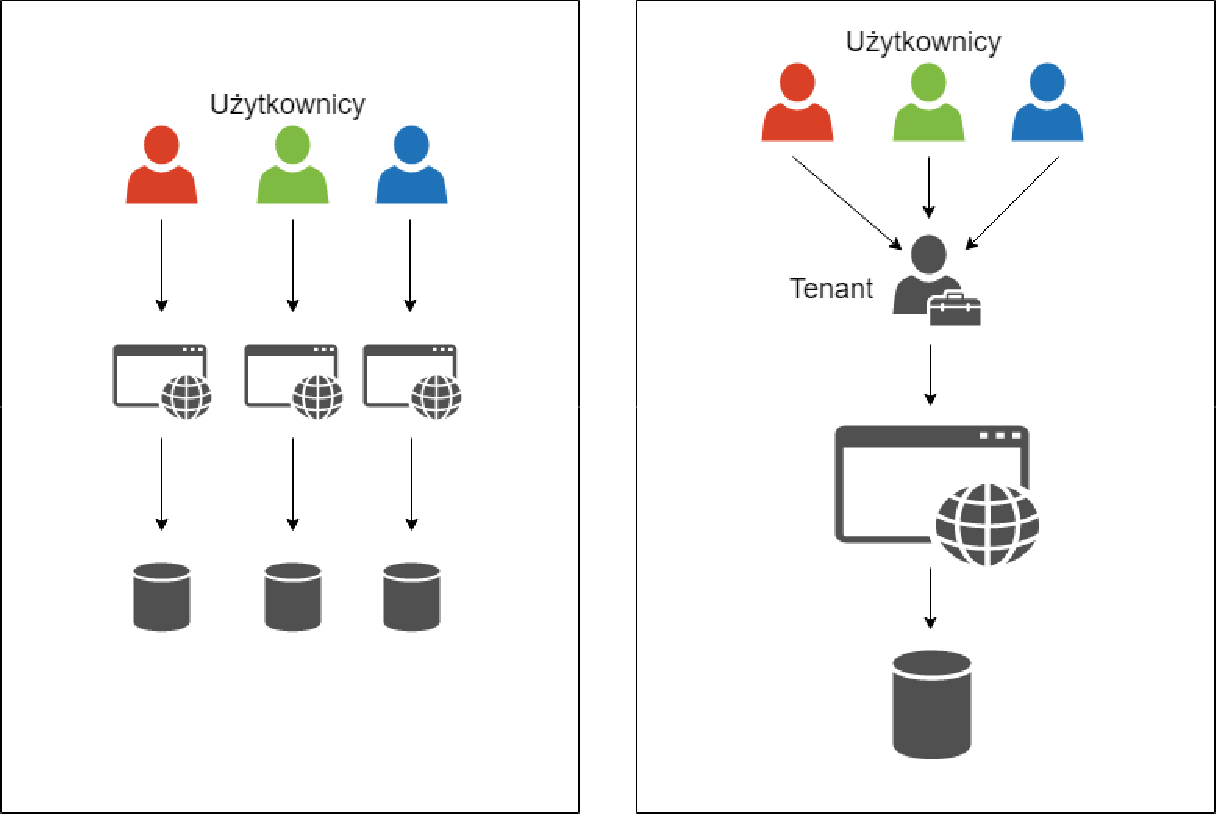
\includegraphics[width=1.0\textwidth]{./img/Multitenancy.pdf}
	\caption{Porównanie zwykłego systemu z wykorzystującym wielotenantowość.}
	\label{id:fig:Multitenancy}
\end{figure}

Aplikację generującą plany lekcji dla szkół można rozwijać w kierunku systemu zarządzającego szkołą. Każdy nauczyciel, logując się do systemu, powinien dostęp do tego samego planu lekcji co inni użytkownicy zgrupowani w ramach tego samego tenanta. Wykorzystanie wielotenantowości jest krokiem naprzeciw rozwojowi aplikacji, może się bowiem pojawić wiele nowych ról użytkowników lub funkcjonalności dostępnych w ramach systemu, które będą dostępne w ramach danej szkoły. Jest to w szczególności przydatne w aplikacjach internetowych, bowiem każdy podmiot korzystający z aplikacji powinien mieć własnego tenanta i własnego administratora w jego obrębie, który może dodawać do swojej grupy nowych użytkowników i przydzielać im uprawnienia.
 
\section{Wzorzec wstrzykiwania zależności}
Wstrzykiwanie zależności (ang. \ang{Dependency Injection}, DI) jest najpopularniejszym wzorcem realizującym koncepcję odwracania sterowania (ang. \ang{Inversion of Control}, IoC). Owa koncepcja polega na przekazaniu zewnętrznemu podmiotowi władzy nad przepływem programu. Najprostszym przykładem jest wykorzystanie wywołań zwrotnych (ang. \ang{callback}) do sterowania przepływem programu. Technika ta jest wykorzystywana często w~interfejsach użytkownika. W~przypadku interfejsu logowania do systemu, klasyczny program zapytałby o~nazwę użytkownika i~hasło, po czym przeszedłby do procedury logowania. Wyposażając taki interfejs w~komponent, który uruchamia wywołanie zwrotne, użytkownik miałby kontrolę nad sterowaniem. Komponentem takim może być zwykły przycisk w~graficznym interfejsie użytkownika. Podstawową ideą wstrzykiwania zależności jest posiadanie zewnętrznego obiektu, który wyposaża elementy systemu w~potrzebne im komponenty \cite{id:IOC_DI_Fowler}. Ponadto, wstrzykiwanie zależności promuje zasadę odwracania zależności (ang. \ang{Dependency Inversion Principle}, DIP) oraz ułatwia zachowanie zasady pojedynczej odpowiedzialności (ang. \ang{Single Responsibility Principle}, SRP) \cite{id:CleanCode}. Zasada odwracania zależności polega na wykorzystywaniu interfejsów zamiast konkretnych implementacji.

Dzięki przekazaniu odpowiedzialności zewnętrznemu podmiotowi przez odwrócenie kontroli, poszczególne elementy systemu nie są bezpośrednio zależne od komponentów z~których korzystają. Ponadto zastosowanie odwracania zależności wraz ze wzorcem wstrzykiwaniem zależności pozwala na podmianę stosownego komponentu na inną jego implementację oraz tworzy luźne powiązania między poszczególnymi elementami. System dzięki temu jest bardziej skalowalny, a~każdy jego element może być oddzielnie testowany. Różnice pomiędzy implementacją niewykorzystującą, a~wykorzystującą wzorzec DI zostały przedstawione na listingu \ref{id:fig:listing:DIvsNonDI}. Przedstawiona sytuacja opisuje klasę wyszukiwkarki książek, która korzysta z~repozytorium książek. W~przypadku niezastosowania wstrzykiwania zależności, taka wyszukiwarka jest całkowicie zależna od repozytorium, którego używa. Dane zapisane są w~plikach tekstowych i~nie ma innej możliwości ich odczytu, takiej jak np. wykorzystanie bazy danych. Ponadto repozytorium tworzone jest w kontekście jednego pliku \lstinline|myBooks.txt|, nie ma możliwości zmiany pliku wejściowego. Należy tą odpowiedzialność przenieść do modułu korzystającego z~wyszukiwarki książek. To tam powinno się precyzować, na jakim zasobie pracuje dana wyszukiwarka. Ponadto należy zapewnić możliwość wykorzystania innych źródeł takich jak baza danych, stosując DIP. Zabieg taki polega na wyodrębnieniu interfejsu i~pośrednio wykorzystaniu jego realizację, co również przedstawia rys. \ref{id:fig:listing:DIvsNonDI}. Na diagramie UML przedstawionym na rys. \ref{id:fig:dipUML} można zauważyć dwie różne realizacje interfejsu \lstinline|BookRepository|. Klasa \lstinline|BookFinder| zależy jedynie od samego interfejsu, dzięki czemu może korzystać z~dowolnej jego implementacji.
\begin{figure}
\begin{lstlisting}
// Bez DI
public class BookFinder {
	private TxtFileBookRepository txtRepository;
	
	public BookFinder() {
		this.txtRepository = new TxtFileBookRepository("myBooks.txt");
	}
}

// Z użyciem DI
public class BookFinder {
	private TxtFileBookRepository txtRepository
	
	public BookFinder(TxtFileBookRepository bookRepo) {
		this.txtRepository = bookRepo;
	}
}

// Z użyciem DI i DIP
public class BookFinder {
	private BookRepository repository
	
	public BookFinder(BookRepository bookRepo) {
		this.repository = bookRepo;
	}
}
\end{lstlisting}
\caption{Porównianie wzorca wstrzykiwania zależności ze standardowym podejściem}
\label{id:fig:listing:DIvsNonDI}
\end{figure}
\begin{figure}
	\centering
	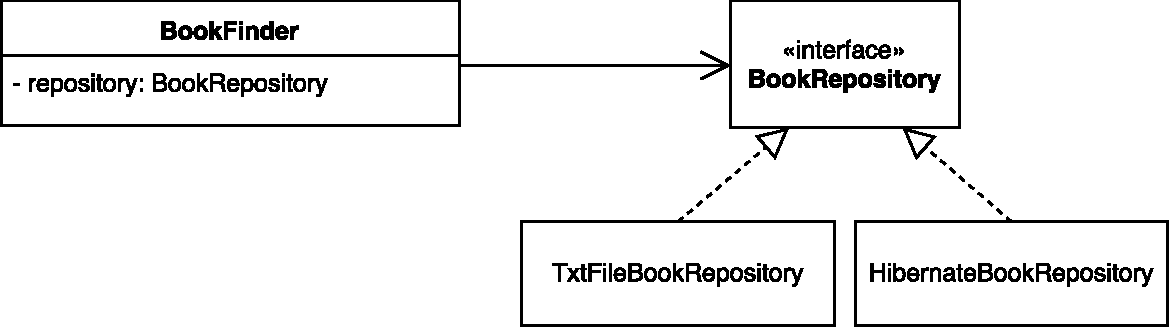
\includegraphics[width=1.0\textwidth]{./img/dipUML.pdf}
	\caption{Zasada odwrócenia zależności}
	\label{id:fig:dipUML}
\end{figure}



\section{Szczegóły implementacji}
\subsection{Opis ważniejszych elementów} %TODO uzupelnic o reszte 
Niniejsza sekcja jest poświęcona opisowi tych klas, które są kluczowe z~punktu widzenia projektowanej aplikacji. Pojawiają się tutaj określenia wzorców wchodzących w~skład technik projektowania sterowanego dziedziną, stąd do zrozumienia pewnych fragmentów konieczna jest wiedza z~sekcji \ref{architekturaDDD} poświęconej tym technikom.

\subsubsection{Struktura wydarzenia}
Wydarzenie kryje się pod klasą \lstinline|ScheduleEvent| i~jest encją korzeniem agregatu. Podstawowymi jej elementami są właściwości wydarzenia, kryjące się pod klasą \lstinline|ScheduleProperty|. Wydarzenie zawiera ich wiele w~postaci kolekcji. Klasa właściwości jest obiektem-wartością i~jej definicję przedstawia listing \ref{id:fig:listing:ScheduleProperty}. Posiada ona nazwę oraz wartość. Przykładowo nazwą może być \lstinline|Sala| a~wartością \lstinline|306|. Aby nadać sens nazwie i~wartości, również opakowano je klasami obiektów-wartości, kolejno \lstinline|SchedulePropertyName| i \lstinline|SchedulePropertyValue|. Ponadto właściwość może być unikalna, dodano zatem flagę \lstinline|nonUnique|, która w~przypadku przyjęcia wartości fałszu wskazuje, że obiekt jest unikalny.
\begin{figure}
\begin{lstlisting}
@ValueObject
@Embeddable
public class ScheduleProperty {

	@Embedded
	@AttributeOverride(name = "name", column = @Column(name = "if_name"))
	private SchedulePropertyName scheduleEntityName;
	
	@Embedded
	private SchedulePropertyValue scheduleEntityValue;
	
	private Boolean nonUnique = false;
}
\end{lstlisting}
\caption{Klasa właściwości wydarzenia}
\label{id:fig:listing:ScheduleProperty}
\end{figure}

Wydarzenie nie przechowuje wszystkich właściwości przez klasę \lstinline|ScheduleProperty|. Przedziały czasowe są zapisywane w~klasie wartości-obiektu takiej jak \lstinline|EventTimeInterval|. Przechowuje ona dzień oraz godzinę rozpoczęcia wydarzenia. Kolejnym ważnym polem jest pole statusu, które jest typu wyliczeniowego. Opisuje ono miejsce w~cyklu życia wydarzenia. Czy jest ono nowe, zagnieżdżone w~harmonogramie, czy może było poddane automatycznej generacji i~wystąpił konflikt. Klasę statusu wraz z~opisami poszczególnych stanów przedstawia listing \ref{id:fig:listing:GenerationStatus}. Kolizja oznacza wystąpienie niespójności lub kolizji warunków.
\begin{figure}
\begin{lstlisting}
public enum GenerationStatus {
	NEW("NOWY"),
	COLLISION("KOLIZJA"),
	NOT_DETERMINABLE("NIEDETERMINOWALNY"),
	ASSIGNED("ZAGNIEZDZONY"),
	UNASSIGNABLE("NIEZAGNIEZDZALNY");
}
\end{lstlisting}
\caption{Status wydarzenia}
\label{id:fig:listing:GenerationStatus}
\end{figure}

Klasa wydarzenia zawiera również raport z~procesu automatycznej generacji. Zapisane są one w~zbiorze obiektów typu \lstinline|PropertyGenerationFailure|. Jest to encja ukryta w~ramach omawianego agregatu. Zawiera ona informacje w~jakich okolicznościach nastąpiła niespójność lub kolizja warunków. Oprócz informacji o~niepowodzeniu, klasa wydarzenia jest w~posiadaniu wszystkich prawidłowych propozycji uzyskanych podczas generacji. Kryją się one pod klasą \lstinline|EventProposal|. Zawiera ona jedynie zestaw właściwości z~proponowanymi wartościami w~formie obiektów typu \lstinline|ScheduleProperty| oraz \lstinline|EventTimeInterval| dla właściwości czasowych wydarzenia.

\subsection{Implementacja mechanizmu generującego harmonogram}
\label{implMechanizmuGen}

Automatyczna generacja harmonogramu na podstawie warunków składa się z~kilku kroków, takich jak wygenerowanie proponowanych zestawów właściwości, wybrania najlepszych z~nich i próby osadzenia wydarzeń w~harmonogramie.  Całość ma miejsce w~klasie \lstinline|ConditionDrivenScheduleGenerator| i~metodzie \lstinline|generate|, która przyjmuje jako parametr trzy kolekcje:
\begin{itemize}
	\item \lstinline|Set<EventTimeInterval>| --- zbiór obiektów przedstawiających ramy czasowe wszystkich możliwych pozycji w~harmonogramie. Jest kolekcją typu \lstinline|Set|, dlatego że istnieje tylko jeden unikalny moment w~czasie, nie mogą wystąpić dwa różne momenty o~takich samych wartościach pól, jak np. \lstinline|środa, godzina 14:30|. Typ \lstinline|Set| zapewnia unikalność obiektów, dodając do niego dwa takie same elementy zostanie przechowany tylko jeden z~nich.
	\item \lstinline|List<ScheduleEvent>| --- zestaw wydarzeń bazowych, czyli takich, których właściwości mechanizm będzie determinował. Wydarzenie takie powinno miec wypełnioną tylko część właściwości, oczekując na zdeterminowanie pozostałych na podstawie warunków. Jest to kolekcja typu \lstinline|List|, dlatego że mogą istnieć dwa dokładnie takie same pod względem właściwości wydarzenia, jak np. dwa elementy, których jedyną wypełnioną właściwością jest przedmiot, np. informatyka. 
	\item \lstinline|Set<ScheduleConditions>| --- zbiór warunków generacji. Podobnie jak w~przypadku elementów reprezentujących ramy czasowe, dwa warunki o~takich samych atrybutach to te same warunki.
\end{itemize}
Przed rozpoczęciem części właściwej mechanizm przygotowuje mapę warunków, której kluczem jest nazwa właściwości determinowanej przez warunek, np. nauczyciel. Algorytm wielokrotnie korzysta z~warunków i~wielokrotne przeszukiwanie całej kolekcji w~celu znalezienia tych, które determinują daną właściwość jest zbędne. Mapa pozwala zwiększyć wydajnośc algorytmu, ponieważ ma niewielką złożoność obliczeniową.

Dla każdego z~podanych wydarzeń bazowych przeprowadzana jest w~pętli procedura wyznaczania propozycji dla wydarzenia. Jest ona zilustrowana na listingu \ref{id:fig:listing:autogeneration1}. Pierwszym krokiem jest konwersja obiektu wydarzenia do klasy \lstinline|EventProposal|, na której pracuje algorytm generujący propozycje, omówiony w~sekcji \ref{rekurencyjny}. Jako, iż wspomniany algorytm można wykorzystać również do generowania propozycji przedziałów czasowych, należy zapisać je w~formie właściwości typu \lstinline|ScheduleProperty|, bowiem główna klasa wydarzenia zapisuje je jako typ \lstinline|EventTimeInterval|. Służy do tego metoda \lstinline|fillWithTimeProperties (EventProposal)|. Po przeprowadzeniu konwersji, mając już niezależną kopię zestawu właściwości wydarzenia bazowego, mechanizm przechodzi do procedury generowania wszystkich prawidłowych zestawów propozycji właściwości dla danego wydarzenia bazowego. Zarówno wyniki jak i~raporty o~niepowodzeniach zapisywane są we wcześniej przygotowanych kontenerach. Jeżeli zbiór niepowodzeń jest pusty a~nie ma żadnych propozycji, oznacza to że wydarzenie jest niedeterminowalne. Jeżeli nie ma propozycji, a~wystąpiły niepowodzenia, oznacza to konflikt typu niespójność lub kolizja warunków. Jeżeli istnieją propozycje, należy zapisać je w~wydarzeniu bazowym.
\begin{figure}
\begin{lstlisting}
for (final ScheduleEvent event : events) {
	EventProposal p = converter.convert(event);
	EventProposal.fillWithTimeProperties(proposal);
	
	Set<EventProposal> results = 
		new HashSet<>();
	Set<PropertyGenerationFailure> failures = 
		new HashSet<>();
		
	conditionDrivenEntityProposer.
		findAllConditionValidEventVariations(
			proposal, determinantes, results, failures );
	
	if(results.isEmpty() && !failures.isEmpty()) {
		event.setGenerationStatus(
				ScheduleEvent.GenerationStatus.COLLISION);
			
		event.setFailures(failures);
		continue;
	}
	else if (results.isEmpty()) {
		event.setGenerationStatus(
				ScheduleEvent.GenerationStatus.NOT_DETERMINABLE);
	}
	else {
		event.setProposals(results);
	}
}
\end{lstlisting}
\caption{Procedura wyznaczania propozycji dla wydarzenia}
\label{id:fig:listing:autogeneration1}
\end{figure}

Po wyznaczeniu wszystkich możliwych propozycji mechanizm przechodzi do drugiego ważnego kroku, mianowicie próby zagnieżdżenia najlepszej propozycji w~harmonogramie. Dzieje się to w~pętli i~tylko dla wydarzeń, które posiadają niepusty zbiór propozycji. Może okazać się, że którakolwiek lub nawet wszystkie propozycje są niemożliwe do zagnieżdżenia, niemniej jednak algorytm próbuje tak długo aż wyczerpie ich zbiór. Zaczyna  od tych, które zostały uznane za najwłaściwsze. Najlepsze rozwiązania algorytm wybiera obliczając pewien współczynnik, którego najmniejsza wartość wskazuje najlepszy zestaw właściwości. Został on opisany w~rozdziale \ref{wspolczynnikAlg}.

Algorytm grupuje zestawy względem współczynników w~mapie, której kluczem jest wartość obliczonego współczynnika. Może bowiem się zdażyć, że kilka zestawów ma równy współczynnik. W~pętli, zaczynając od najniższego współczynnika mechanizm próbuje wstawić takie wydarzenie do harmonogramu. Jeżeli istnieje kilka zestawów o~równym współczynniku, wybierane są według kolejności. Cały proces próby wstawienia wydarzenia ilustruje listing \ref{id:fig:listing:autogeneration2}. Jest to okrojona wersja oryginalnej metody, ze względu na dużą ilość kodu. Z~mapy współczynników wybierany jest zestaw o~najniższym współczynniku. Dla każdego elementu zestawu sprawdzane jest, czy przydzielono właściwościom czasowym wartości. Jeżeli nie lub są niekompletne, należy wybrać jakiś przedział czasowy, który będzie wolny i~zgodny z~warunkami. Służy temu metoda \lstinline|tryFindingValid Intervals| klasy \lstinline|ConditionAwareTimeProposer|. Jeżeli nie znaleziono żadnego przedziału, oznacza to że zabrakło miejsca w~harmonogramie lub właściwości propozycji kolidują z~wolnymi terminami. W~takim wypadku wybierana jest następna propozycja zestawu właściwości, aż do ich wyczerpania. Jeżeli żadna z~propozycji nie zostanie zagnieżdżona w harmonogramie, nie dojdzie do ustawienia flagi \lstinline|succesfullyAdded|. Po wyjściu z~całej procedury wydarzenie główne zostanie oznaczone statusem \lstinline|NIEZAGNIEŻDŻALNY|. Jeżeli któraś z~propozycji zostanie jednak osadzona, procedure należy przerwać, dlatego w~każdej pętli w~odpowiednich miejscach sprawdzana jest wspomniana flaga, czy udało się zagnieździć wydarzenie i~w~przypadku sukcesu, przerywa się kolejne iteracje.
\begin{figure}
\begin{lstlisting}
boolean succesfullyAdded = false;
Map<Double,Set<EventProposal>> ratio =
		calculateRatio(schedule, propositions);
		
for(int i = 0; i< ratio.keySet().size(); i++ ) {
	Double currentMin = 
			Collections.min(ratio.keySet());
	Set<EventProposal> minProposals = 
			ratio.get(currentMin);
			
	for (EventProposal minProposal : minProposals) {
		if(!minProposal.hasFullTimeSpecified()) {
		
			Set<EventTimeInterval> intervals = 
				conditionAwareTimeProposer.tryFindingValidIntervals(
					schedule, determinantes, minProposal);
			
			if(intervals.isEmpty()) {
				continue;
			}
			tryAddingForIntervals(intervals, minProposal)) 
				succesfullyAdded = true;
			}
		}
		else {
			if(!consistencyChecker.canAddToSchedule(minProposal)){
				continue;
			}
			
			// dodawanie do harmonogramu
			succesfullyAdded = true;
		}
		
		if(succesfullyAdded) {
			break;
		}
	}
	
	if(succesfullyAdded) {
		break;
	}
	
	ratio.remove(currentMin);
}

if (!succesfullyAdded) {
	eventWithPropositions.setGenerationStatus(
			ScheduleEvent.GenerationStatus.UNASSIGNABLE);
}
\end{lstlisting}
\caption{Procedura wybierania i zagnieżdżania najlepszych propozycji}
\label{id:fig:listing:autogeneration2}
\end{figure}




\subsection{Algorytm generujący propozycje wydarzeń}
\label{rekurencyjny}

Algorytm generujący jest algorytmem rekurencyjnym i~wyczerpującym, ponieważ sprawdza każdą możliwość. Jako argumenty przyjmuje bazowe wydarzenie w~formie obiektu klasy \lstinline|EventProposal|, referencję do kontenera wyników tego samego typu, referencję do konterera raportów o~niepowodzeniach klasy \lstinline|PropertyGenerationFailure| i~ostatecznie mapę warunków, w~której kluczem jest nazwa warunku. Podczas wywołania algorytmu, zanim przejdzie on w~tryb rekurencyjny, weryfikowane są właściwości. Jeżeli żadna z nich nie posiada wartości to nie ma punktu odniesienia dla warunków. Wydarzenie jest wtedy niedeterminowalne i~dalsze operacje nie są wymagane. W~innym wypadku, wywoływana jest część właściwa. Całość części wstępnej prezentuje listing \ref{id:fig:listing:b4Recursion}. Wartość fałszu przekazana do części właściwej została omówiona w~dalszej części rozdziału.
\begin{figure}
\begin{lstlisting}
public void findAllConditionValidEventVariations(
	EventProposal baseEvent,
	Map<SchedulePropertyName, Set<ScheduleCondition>> determinantes,
	Set<EventProposal> results,
	Set<PropertyGenerationFailure> generationFailures) {
	
	if (generatorExtractingFacade.hasOnlyUnsetEntities(
				baseEvent.getEntities())) {
		return;
	}
	
	this.findAllConditionValidEventVariations(baseEvent, determinantes, results, false, generationFailures);
}
\end{lstlisting}
\caption{Weryfikacja konieczności wykonania algorytmu}
\label{id:fig:listing:b4Recursion}
\end{figure}

Okrojona wersja kodu części właściwej jest przedstawiona na listingu \ref{id:fig:listing:recursion}. Pierwszym krokiem części właściwej jest walidacja właściwości pod kątem konfliktów. Jeżeli występuje ich niespójność lub istnieje kolizja warunków, metoda jest przerywana i~następuje wyjście z~danego poziomu rekurencji. Jeżeli właściwości nie zawierają konfliktów, należy sprawdzić czy istnieją jakieś nieustalone wartości wśród właściwości, a~gdy istnieją, to czy te właściwości posiadają jakiekolwiek determinanty. Nie znajdując takich, należy wykorzystać informację przekazaną z~wyższego poziomu rekurencji, którą jest flaga \lstinline|wasModified|. Jest ona zainicjalizowana wartością fałszu, przed rozpoczęciem części właściwej, jak przedstawiono na listingu \ref{id:fig:listing:b4Recursion}. Zostaje ona zmieniona na wartość prawdy tylko gdy zdeterminowano przynajmniej jedną wartość właściwości. Sprawdzenie tej flagi pozwala na zdecydowanie, czy zestaw właściwości można dodać do kontenera wyników. Jeżeli nie było konfliktów i~nie da się wyznaczyć innych właściwości, oznacza to że wyczerpano już zasoby. Jednakże taka sytuacja może się zdarzyć, gdy podamy niedeterminowalne i~niekonfliktowe wydarzenie bazowe. Na pierwszym poziomie rekurencji zostanie potwierdzone, że właściwości są prawidłowe i~wyczerpano zasoby. Taki zestaw zostaje dodany do wyników, mimo że nie została wygenerowana ani jedna wartość właściwości. Wspomniana flaga jest strażnikiem, który temu zapobiega. Należy pamiętać, że nie jest ona referencją, a~zwykłą wartością. Nie jest zatem globalna w~całej procedurze.

W~przypadku gdy znaleziono determinowalne właściwości o~nieustalonej jeszcze wartości, to dla każdej z~nich generowany jest zbiór wartości, które wymuszają warunki. Jeżeli kilka warunków wymusza wartość tej właściwości, brana pod uwagę jest ich część wspólna. Taki zbiór nie może być pusty, dlatego że na początku metody sprawdzane są właściwości pod kątem konfliktów. Jeżeli zbiór jest pusty to musiała nastąpić kolizja warunków. Dla każdej wartości ze zbioru wywoływana jest kolejna rekurencja, po uprzednim uzupełnieniu zestawu właściwości o~nową wartość. Jeżeli kolejne stopnie rekurencji wykryją konflikt to propozycja nie zostanie dodana do kontenera wyników. Po powrocie z rekurencji, która została właśnie była wywołana, następuje powrót z~aktualnego poziomu, lub wejście w~rekurencję dla kolejnej wartości ze zbioru.

Dodawanie do wyników ma miejsce tylko na początku metody po walidacji ich poprawności, ale omijając blok, w~którym następuje determinacja właściwości. Propozycja zestawu będzie dodana do wyników dopiero wtedy, gdy zestaw będzie niekonfliktowy i niedeterminowalny oraz na którymś z~wyższych poziomów rekurencji zdeterminowano jakąkolwiek właściwość, ponieważ jeżeli nie można zdeterminować żadnej właściwości, a~we~wcześniejszych poziomach rekurencji się to udało, to oznacza to, że wyczerpano zasoby i~nie doszło do porażki. Algorytm nie wchodzi wtedy w~blok odpowiedzialny za wyznaczanie kolejnych propozycji właściwości, ale sprawdza wartość flagi \lstinline|wasModified| i~dodaje propozycję do kontenera.
\begin{figure}
\begin{lstlisting}
if (!arePropertiessValid(baseEv,conditions,failures)){
	return;
}

Set<ScheduleProperty> unsetDeterminableProperties = 
		generatorExtractingFacade
			.unsetDeterminablePropertiesOf(baseEv,conditions)

if (!unsetDeterminableProperties.isEmpty()) {
				
	for(ScheduleProperty unsetProperty : unsetDeterminableProperties) {

		Set<SchedulePropertyValue> inCommonValues = 
				generatorExtractingFacade
						.prepareInCommonPropositionsForPropertyInEvent(
								baseEv, conditions, unsetProperty);

		for (SchedulePropertyValue val : inCommonValues) {
			EventProposal copy = new EventProposal(baseEv);
			copy.getProperties().remove(unsetProperty);
			copy.getProperties().add(new ScheduleProperty(unsetProperty.propertyName(), val));

			wasModified = true;
			findAllConditionValidEventVariations(copy, conditions, results, wasModified, generationFailures);
		}	
	}
} else {
	if (wasModified) {
		results.add(baseEv);
	}
}

\end{lstlisting}
\caption{Część właściwa algorytmu rekurencyjnego}
\label{id:fig:listing:recursion}
\end{figure}


\subsection{Implementacja architektury sterowanej zdarzeniami}

Mechanizm obsługi zdarzeń w tworzonej aplikacji został zaprojektowany zgodnie z następującymi wymaganiami co do sposobu działania:%TODO czy to do rozdz. 3 Wymagania niefunkcjonalne? % KS: Jeszcze zobaczymy.
\begin{itemize}
	\item pojedynczy odbiorca może przetwarzać wiele typów zdarzeń;
	\item kilka różnych odbiorców może przetwarzać ten sam, wspólny dla siebie typ zdarzenia;
	\item zdarzenie musi być dostarczone do każdego zainteresowanego nim odbiorcy;
	\item zdarzenie nieposiadające zainteresowanych odbiorców jest neutralne dla systemu.
\end{itemize}
Wymagania techniczne:
\begin{itemize}
	\item zdarzenie jak i odbiorca muszą być oznaczone odpowiednią adnotacją, klasą abstrakcyjną lub interfejsem;
	\item odbiorca przetwarza zdarzenia w metodzie \lstinline|handle|, przyjmującą dokładnie jeden argument, który jest instancją typu oznaczonego jako zdarzenie;
	\item zdarzenie jak i odbiorca mogą być rozszerzane w hierarchii abstrakcji. Opublikowanie zdarzenia konkretnego nie skutkuje obsługą zdarzenia klasy rodzica;
	\item opublikowane zdarzenie jest objęte transakcją --- musi zostać przetworzone, jeżeli posiada odbiorców;
	\item opublikowane zdarzenie jest odporne na awarie systemu i jest odtwarzane po jego ponownym uruchomieniu;
	\item korzystanie z funkcjonalności tego systemu powinno wymagać jedynie implementacji odbiorcy i utworzenia klasy zdarzenia;
	\item system powinien być autokonfigurowalny, nie wymagając manualnego ustawiania czy modyfikacji sieci komunikacyjnej.
\end{itemize}

Zaprojektowany system przedstawia rysunek \ref{id:fig:6}. Interfejs \lstinline|Event| jest pusty i oznacza klasę jako zdarzenie. Brak jakichkolwiek cech i metod sugeruje wykorzystanie adnotacji, te jednak w języku Java nie pozwalają na wymuszenie implementacji innych interfejsów lub rozszerzania klas abstrakcyjnych. Jako że system przesyła zdarzenia jako zserializowane obiekty, zdarzenie musi realizować interfejs \lstinline|Serializable|. Interfejsy mogą implementować inne interfejsy i jest to zależność przechodnia. Każda klasa oznaczona jako zdarzenie jest zatem obsługiwana przez mechanizmy serializacji Javy.

\begin{figure}
	\centering
	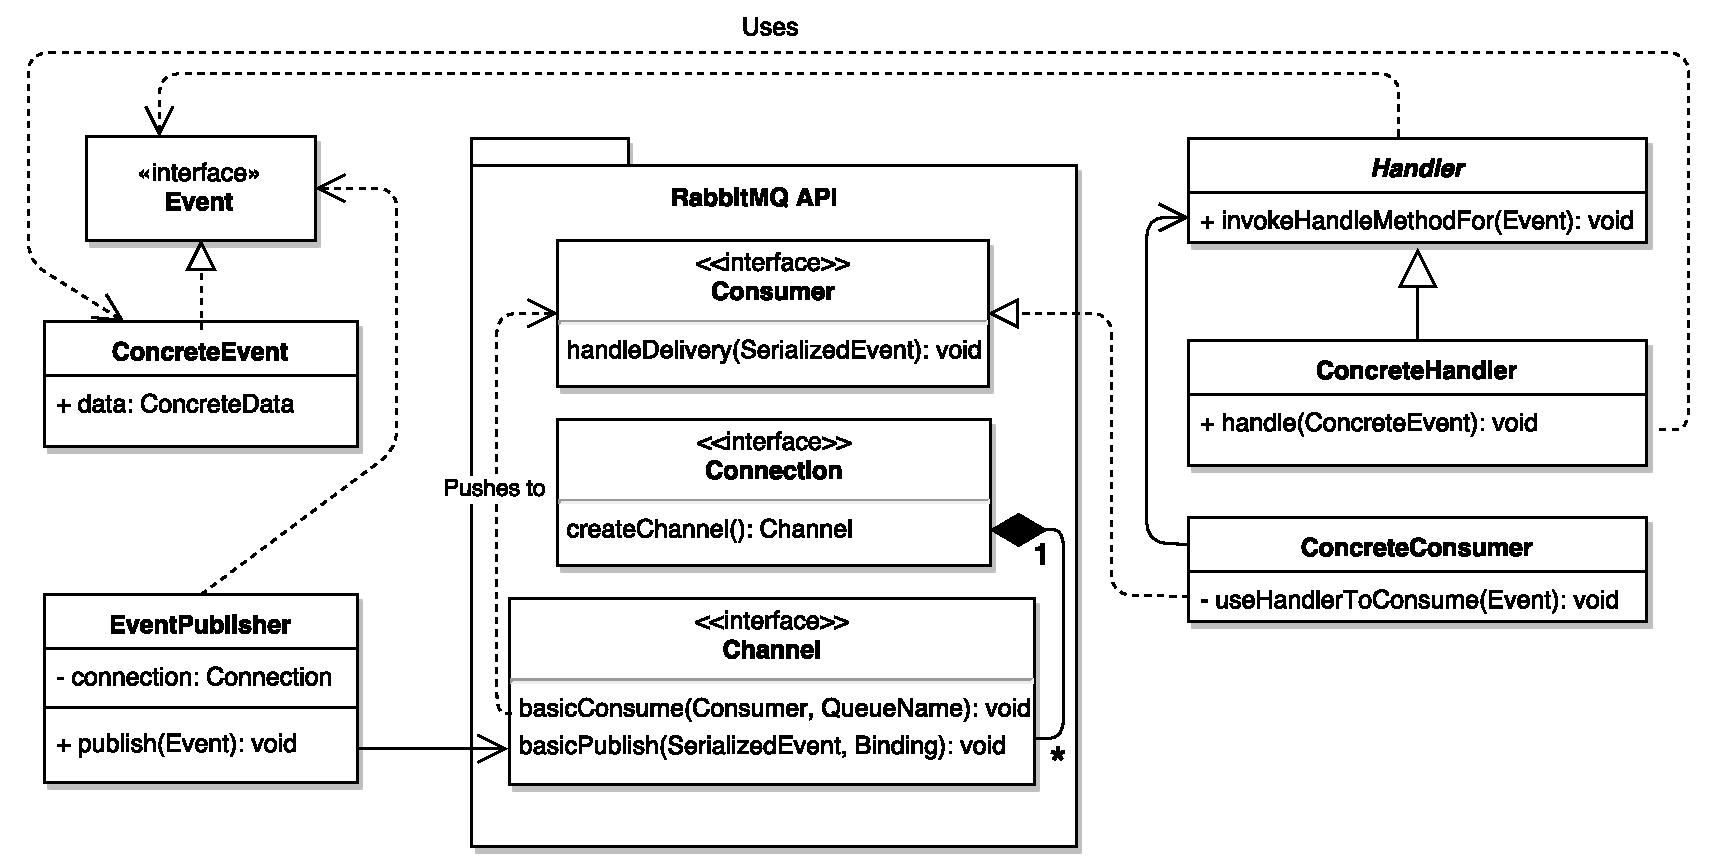
\includegraphics[width=1.0\textwidth]{./img/EDA_Rabbit_UML.pdf}
	\caption{Uml}
	\label{id:fig:6}
\end{figure}
Omówienia wymaga realizacja interfejsu \lstinline|Event| przez klasę \lstinline|ConcreteEvent| na rys. \ref{id:fig:6}. Zawiera ona pole tylko do odczytu typu \lstinline|ConcreteData|. Cechą zaprojektowanego mechanizmu jest dowolność w implementacji klasy zdarzenia. Widoczność klas w ramach jednej aplikacji pozwala odbiorcy na bezpośrednie ich użycie, co za tym idzie, w kontekście aplikacji nie jest wymagane kodowanie wiadomości w odpowiednim formacie i dekodowanie ich przez odbiorcę. Jeżeli obie warstwy, zarówno generująca jak i przetwarzająca, posiadają dostęp do wygenerowanej klasy, nie potrzebne jest standaryzowanie formatu wiadomości. W przeciwnym przypadku wymagana jest znajomość struktury wiadomości. Można do tego wykorzystać popularny format tekstowy \lstinline|JSON|, czy język znaczników \lstinline|XML|. Listing na rys. \ref{id:fig:listing:EventHandlerRelation} przedstawia omawianą sytuację na przykładzie zdarzenia opłacenia faktury:

\begin{figure}
	\begin{lstlisting}
public class InvoicePaid implements Event {
	public final InvoiceData invoiceData;
}

public class InvoiceHandler extends Handler {
	public void handle(InvoicePaid event) {
	int invoiceNum = event.invoiceData.getNumber();
	String email = event.invoiceData.getCustomerEmail();

	Database.markInvoiceAsPaid(invoiceNum);
	EmailService.sendPaymentConfirmationTo(email))
	}
}
	\end{lstlisting}
	\caption{Relacja elementu obsługującego z klasą zdarzenia}
	\label{id:fig:listing:EventHandlerRelation}
\end{figure}
Odbiorca \lstinline|InvoiceHandler| może bezpośrednio korzystać z zawartości klasy zdarzenia \lstinline|InvoicePaid|. W~przypadku gdy warstwa przetwarzająca nie posiada danych o tej klasie, konieczna jest znajomość struktury wiadomości. Na jej podstawie należy dokonać analizy i~wydobycia zainteresowanych danych z~odebranej wiadomości, bądź utworzenie dodatkowej klasy na podstawie znanej struktury, o~ile jest ona stała.
%TODO oznaczyc na rysunku concrete event jako final
Wykorzystane oprogramowanie RabbitMQ posiada prosty interfejs, za pomocą którego można skonfigurować całą sieć komunikacyjną. Autokonfigurowalność zapewniono poprzez użycie narzędzia z paczki \lstinline|org.reflections|. Za cały proces autokonfiguracji odpowiedzialna jest klasa \lstinline|HandlerRegistrar| dostępna w źródłach programu. Wspomniane narzędzie pozwala na pobranie wszystkich klas rozszerzających klasę \lstinline|Handler| w ramach aplikacji.
\begin{lstlisting}
Set<Class<? extends Handler>> classes = 
new Reflections("").getSubTypesOf(Handler.class);
\end{lstlisting}
Mechanizm refleksji Javy umożliwia ekstrakcję typów parametrów w metodzie \lstinline|handle(ConcreteEvent)|. Dzięki temu możliwe jest skompletowanie informacji o~wszystkich odbiorcach oraz zdarzeniach o~których chcą być informowani.
\begin{lstlisting}
Method handleMethod = handlerClazz.getDeclaredMethods();
Class<?>[] events = handleMethod.getParameterTypes();
\end{lstlisting}

Posiadając taki zestaw informacji, tworzony jest jeden punkt wymiany typu \lstinline|direct| oraz tyle kolejek, ile istnieje klas rozszerzających klasę \lstinline|Handler|. Klucze wiążące kolejki z konsumentami to zbiory nazw klas zdarzeń. Każda kolejka może mieć wiele kluczy. Podczas publikowania zdarzenia do usługi RabbitMQ pobierana jest jego nazwa, która stanowi wiązanie, a każda kolejka posiadająca klucz o takiej wartości odbierze to zdarzenie. Do pojedynczej kolejki przyłączony jest minimum jeden konsument (interfejs \lstinline|Consumer|) pracujący w ograniczonej puli wątków. Konsumenta należy zaprogramować tak by wykonywał pożądane przez nas operacje. W tym przypadku wystarczy przydzielić do konsumenta odbiorcę i wywołać jego metodę \lstinline|handle(Event)|.

Nietrywialnym sposobem na uzyskanie wygody, dzięki której tworząc odbiorcę wymaga się jedynie utworzenia prostej metody, a~utworzenie zdarzenia tylko implementacji odpowiedniego interfejsu --- jest podniesienie poziomu abstrakcji oraz wykorzystanie refleksji. Jak przedstawia rysunek \ref{id:fig:6}, konsument ma referencję do odbiorcy w postaci wiązania późnego i wywołuje metodę, której parametrem jest zdarzenie również w formie wiązania późnego. Brak abstrakcyjnego odbiorcy wymagałby manualnego definiowania wielu klas konsumentów oraz wyposażenia ich w logikę postępowania w zależności od odebranego zdarzenia. Oprócz rażącej niewygody łamana jest zasada odwracania zależności. Klasa abstrakcyjna \lstinline|Handler| natomiast pozwala na wykonanie jednej prostej operacji
\begin{lstlisting}
public class ConcreteConsumer implements Consumer {
	private Handler handler;
	public void handleDelivery(Event e) {
		this.handler.handle(e)
	}
}
\end{lstlisting}
Problemem jest jednak uzależnienie abstrakcji od jej klas konkretnych. Logika przetwarzania zdarzeń znajduje się bowiem w klasach rozszerzających \lstinline|Handler| i~nie jest dostępna z~poziomu klasy rodzica. Aby rozwiązać ten problem, wystarczy wykorzystać refleksję do pobrania z odbiorcy jego metod i wywołać odpowiednią dla odebranego zdarzenia. Listing na rys. \ref{id:fig:listing:RabbitAbstractHandlerUsage} przedstawia realizację tego rozwiązania. Metoda \lstinline|handle(Event)| przyjmuje jako parametr instancję zdarzenia i przy pomocy metody \lstinline|getClass{}| pobiera obiekt reprezentujący jego klasę konkretną. Następnie posiłkując się słowem kluczowym \lstinline|this| pobierany jest obiekt klasy konkretnej odbiorcy przetwarzającego zdarzenie, a z niego obiekt reprezentujący metodę \lstinline|handle(ConcreteEvent)|, gdzie parametr jest typem zdarzenia który pobrano chwilę wcześniej. Mając obiekt metody, można ją wywołać na dowolnej instancji obiektu, podając zestaw parametrów, który w tym przypadku zawiera tylko instancję obiektu zdarzenia do przetworzenia. Opisany proces ilustruje listing na rys. \ref{id:fig:listing:RabbitAbstractHandlerUsage}.
\begin{figure}
	\begin{lstlisting}
public abstract class Handler {
	protected <E extends Event> void handle(E e) {
		Class[] params = new Class[] { e.getClass() };
		Method m = this.getClass().getDeclaredMethod("handle", params);	
		m.invoke(this, e)
	}
}
	\end{lstlisting}
	\caption{Wywołanie implementacji metody obsługującej z poziomu klasy abstrakcyjnej}
	\label{id:fig:listing:RabbitAbstractHandlerUsage}
\end{figure}

\subsection{Wstrzykiwanie zależności przez bibliotekę Spring}

Biblioteka Spring może pełnić funkcję kontenera IoC, który jest odpowiedzialny za wstrzykiwanie zależności. Chodzi o~dostarczenie danym obiektom instancji klas, które powinny być do nich wstrzyknięte. Takowy kontener znacznie upraszcza realizację wzorca wstrzykiwania zależności. Pozwala on zmniejszyć ilość kodu oraz uczynić go czytelnym i~klarownym, różnicę między zwykłym wstrzykiwaniem zależności, a~takim wykorzystującym kontener można zaobserwować na listingu \ref{id:fig:listing:DiWithAndWithoutIoC}. Dzięki kontenerowi nie jest konieczne manualne tworzenie nowych instancji wstrzykiwanych komponentów. Spring wykorzystuje drzewa i~grafy do ułożenia struktury zależności, po czym tworzy wszystkie komponenty sam. Wystarczy je pobrać z kontenera, który jest zwany kontekstem. Na przedstawionym listingu wykorzystano sposób mapowania zależności poprzez adnotacje. Istnieje także możliwość skonfigurowania poszczególnych komponentów w~plikach xml. Każdy komponent musi być oznaczony adnotacją \lstinline|Component|, jak przedstawiono na listingu. Adnotację tę można zastąpić jedną z~kilku innych, bardziej pasujących do kontekstu. Ich użycie nie ma wpływu na wynik, są praktycznie wykorzystywane jedynie w~celach informacyjnych. Należą do nich \lstinline|Repository|, \lstinline|Service|, \lstinline|Controller|. W~przypadku oznaczania klasy realizującej dostęp do bazy danych (repozytoria), sensownym będzie użycie odpowiednika o~nazwie \lstinline|Repository|.
\begin{figure}
\begin{lstlisting}
	// Bez kontenera IoC
	public class SomeClass {
		... 
		public SomeClass(ComponentA a, ComponentB b, ...){
			this.a = a;
			this.b = b;
			...
		}
	}
	
	SomeClass obj = new SomeClass(new ComponentA(args), new ComponentB(args), ...);
	
	// Z użyciem kontenera biblioteki Spring
	@Component
	public class SomeClass {
		@Autowired
		private ComponentA a;
		@Autowired
		private ComponentB b;
		...
	}
	
	SomeClass obj = ctx.getBean(SomeClass.class);
\end{lstlisting}
\caption{Wstrzykiwanie zależności z kontenerem IoC i bez}
\label{id:fig:listing:DiWithAndWithoutIoC}
\end{figure}

Użycie kontenera nie jest jednak sprawą tak prostą, jak mogło by się wydawać. Komponenty mogą być wstrzykiwane jedynie do klas, które same są komponentami. Ponadto, wstrzykiwanie nie zadziała, gdy komponent jest tworzony poprzez użycie operatora \lstinline|new|. Bowiem nie miałoby to większego sensu, jeżeli odpowiedzialność za tworzenie tych obiektów jest powierzana Springowi. Wyjątkiem stanowią elementy oznaczone adnotacją \lstinline|Configurable|, omówione w~dalszej części rozdziału. Dany komponent można pobrać jedynie z~kontenera, który w~Springu nazywany jest kontekstem. Kontekst należy poinstruować, które paczki z~kodem źródłowym ma przeskanować, w~celu znalezienia i~utworzenia odpowiednich obiektów z~ich zależnościami. Aby to zrobić, trzeba utworzyć klasę konfiguracyjną i~opatrzyć ją adnotacją \lstinline|Configuration| oraz \lstinline|ComponentScan|. Ta ostatnia może posiadać argument będący nazwą paczki, którą Spring przeskanuje razem z~paczkami podrzędnymi. Jeżeli taki argument nie zostanie podany, skanowanie odbędzie się w~obrębie paczki do której należy klasa opatrzona omawianą adnotacją, wraz z~paczkami podrzędnymi. W~przypadku konstruowanej aplikacji, klasą konfiguracyjną jest serwlet inicjalizujący omówiony w~innym rozdziale. Zaznaczono, aby skanowanie odbyło się w~obrębie nadrzędnych paczek projektu, takich jak \lstinline|com.scheduler| oraz \lstinline|com.configuration|.

Wielce nieeleganckim jest pobieranie każdego komponentu z~osobna za pomocą metody \lstinline|getBean(Class<T>)|, którą zaprezentowano na rysunku \ref{id:fig:listing:DiWithAndWithoutIoC}. Zabieg ten powinno się wykonywać jedynie podczas inicjalizowania nadrzędnych komponentów w~hierarchii zależności. Każde podrzędne komponenty zawierające się w~komponencie źródłowym, który uzyskano poprzez metodę pobierającą komponent z~kontekstu, będą wstrzyknięte przez Spring. Będą one mogły wtedy do woli wstrzykiwać inne komponenty. Ważnym jest jedynie, aby dany obiekt był pobrany z~kontenera lub należał do obiektu, który był w~ten sposób zainicjalizowany. Istnieją jednak pewne klasy, których obiekty wymagają inicjalizacji poprzez operator \lstinline|new|, ze względu na swoją specyfikę. W~konstruowanym narzędziu są to klasy widoków, które znacznie wygodniej jest obsługiwać, jak również odbiorcy zdefiniowani w~ramach architektury sterowanej zdarzeniami. Odbiorca taki wymaga komponentów realizujących pewne operacje i~udostępniających pewne dane, np. chcąc zapisać coś do bazy danych będzie potrzebował repozytorium, które też jest komponentem. Jako że odbiorcy są inicjalizowani przez specjalny mechanizm, który tworzy ich instancje poprzez metodę \lstinline|newInstance()|, nie są oni częścią kontenera. W~tej sytuacji należy wykorzystać adnotację \lstinline|Configurable|, która pozwala na wstrzykiwanie zależności do klas nie wchodzących w~skład kontenera. Wymaga to poinformowania Springa o~możliwości wykonywania takich operacji, poprzez oznaczenie klasy konfiguracyjnej kolejną adnotacją, mianowicie \lstinline|EnableSpringConfigured|. Koniecznym jest także odblokowanie mechanizmów aspektowego programowania Springa. Ze względu na to, że inicjalizacja odbiorców odbywa się podczas działania programu, działanie tych mechanizmów tylko podczas kompilacji nie wystarczy. Należy zatem użyć adnotacji \lstinline|EnableLoadTimeWeaving|. Finalnie klasa konfiguracyjna powinna być oznakowana tak jak przedstawia listing \ref{id:fig:listing:ConfigurationSpring}.
\begin{figure}
\begin{lstlisting}
@Configuration
@ComponentScan({"com.scheduler", "com.configuration"})
@EnableSpringConfigured
@EnableLoadTimeWeaving(aspectjWeaving = EnableLoadTimeWeaving.AspectJWeaving.ENABLED)
public class SpringConfigurationClass {
	...
}
\end{lstlisting}
\caption{Adnotacje klasy konfigurującej kontekst Springa}
\label{id:fig:listing:ConfigurationSpring}
\end{figure}

\subsection{Realizacja koncepcji projektowania sterowanego dziedziną}
Głównymi technikami projektowania sterowanego dziedziną jest odpowiedni podział na warstwy oraz wyznaczenie granic odpowiedzialności poszczególnych elementów systemu. Dokonuje się tego poprzez zastosowanie wzorców komponentów budujących model dziedziny nazywanych cegiełkami. Do standardowych warstw wprowadzono dodatkową, mianowicie oddzielono od warstwy interfejsów warstwę prezentacji. Wprowadzono taki zabieg, ponieważ warstwa prezentacji często jest utożsamiana z~warstwą interfejsów. Aby zwiększyć skalowalność systemu, zdecydowano się na rozdzielenie tych odpowiedzialności pomiędzy dwie odrębne warstwy. Na rys. \ref{id:fig:warstwy} zilustrowano podział na paczki w~projekcie aplikacji. W~każdej z~warstw zawierają się paczki dotyczące danych obszarów dziedziny systemu. Najważniejszymi obszarami są poszczególne właściwości harmonogramu (nauczyciele, sale itd.), sam harmonogram, wydarzenia w~nim występujące oraz warunki automatycznej generacji. Na ilustracji można również zauważyć paczkę przeznaczoną na zdarzenia powiązane z~danym obszarem dziedzinowym.
\begin{figure}
	\centering
	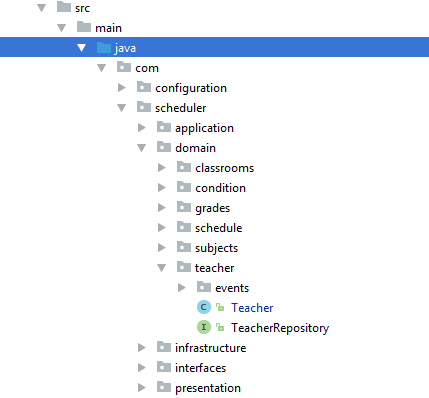
\includegraphics[height=0.4\textheight]{./img/strukturaDDD.png}
	\caption{Podział na warstwy}
	\label{id:fig:warstwy}
\end{figure}

W~celu oznaczenia cegiełek DDD utworzono kilka pomocniczych, czysto informacyjnych adnotacji takich jak \lstinline|AggregateRoot|, \lstinline|ValueObject|, \lstinline[literate={S}{S}{0\discretionary{-}{}{}}]|ApplicationService|, \lstinline|DomainService|. Najważniejszym agregatem w~aplikacji jest klasa \lstinline[literate={d}{d}{0\discretionary{-}{}{}}]|ScheduleEvent|. Posiada ona referencje do takich encji jak \lstinline|EventProposal| i~\lstinline[literate={t}{t}{0\discretionary{-}{}{}}]|PropertyGenerationFailure|. Dodatkowo, \lstinline|PropertyGenerationFailure| sam jest agregatem. Jest on klasą posiadającą informacje o~konfliktach oraz zawiera referencję na wydarzenie, podczas którego generowania owe konflikty wystąpiły. Cała ta klasa jest ukryta w~agregacie a~informacje jakie nosi są dostępne jedynie z~jego poziomu. Usuwając obiekt wydarzenia, usuniemy również informacje na temat konfliktów, które wystąpiły podczas jego generacji, oraz proponowanych zestawach właściwości, które otrzymano w~procesie automatycznego generowania. Definicję klasy wydarzenia przedstawiono na listingu \ref{id:fig:listing:ScheduleEventAggregate}. Widać na nim mapowanie obiektowo-relacyjne. Odpowiednie adnotacje mapujące pozwalają sprecyzować co ma się stać ze~zmapowanymi encjami, gdy agregat zostanie usunięty. Można również zaobserwować informacyjne oznaczenie klasy adnotacją \lstinline|AggregateRoot|. Omawiana klasa składa się nie tylko z~encji ale również obiektów-wartości takich jak \lstinline|EventTimeInterval|, który opisuje dzień i~godzinę wystąpienia zdarzenia. Obiekty-wartości są łatwe w~mapowaniu obiektowo-relacyjnym, ponieważ wystarczy użyć adnotacji \lstinline|Embedded|. Nie wymagają one bowiem swojej własnej tabeli w~bazie oraz unikalnego identyfikatora. Agregat ten również posiada prostą logikę biznesową której nie przedstawiono na listingu. Między innymi pozwala na sprawdzenie, czy wydarzenie ma jakieś konflikty.
\begin{figure}
	\begin{lstlisting}
	@AggregateRoot
	@Entity
	@Table(name = "schedule_events")
	public class ScheduleEvent implements TenantAware {
	@Id
	@GeneratedValue
	private long id;
	
	@Embedded
	private EventTimeInterval timeInterval;
	
	@ElementCollection
	@CollectionTable(name = "properties2event")
	private Set<ScheduleProperty> scheduleProperties;
	
	@Enumerated(EnumType.STRING)
	@Column(nullable = false)
	private GenerationStatus generationStatus;
	
	@OneToMany(cascade = CascadeType.ALL)
	@JoinColumn(name = "proposalId")
	private Set<EventProposal> proposals;
	
	@OneToMany(cascade = CascadeType.ALL)
	@JoinColumn(name = "failureId")
	private Set<PropertyGenerationFailure> failures;
	
	@Embedded
	private TenantId tenantId;
	...
	}
	\end{lstlisting}
	\caption{Klasa wydarzenia będąca korzeniem agregatu}
	\label{id:fig:listing:ScheduleEventAggregate}
\end{figure}

Przykładem serwisu domenowego może być klasa \lstinline[literate={C}{C}{0\discretionary{-}{}{}}]|ScheduleConsistencyChecker|, jest ona odpowiedzialna za sprawdzanie czy dodanie do harmonogramu wydarzenia o~pewnych właściwościach jest możliwe. Jest ona serwisem domenowym encji ukrytej w~agregacie wydarzenia. Mianowicie jest to klasa \lstinline|EventProposal|. Serwis ten jest też pośrednio wykorzystywany do sprawdzania czy obiekt klasy \lstinline|ScheduleEvent| może być osadzony w~harmonogramie, potrzebna jest jedynie jego konwersja do tymczasowego obiektu typu \lstinline|EventProposal|. Omawiany serwis jest bezstanowy, jak należy czynić.

Kwintesencją wszystkich elementów DDD są serwisy aplikacyjne. Najważniejszym z~nich jest sam generator, który łączy kilka innych serwisów domenowych, a~nawet aplikacyjnych. Jest to klasa \lstinline|ConditionDrivenScheduleGenerator|, wykorzystuje ona serwisy wyszukujące konflikty, wyszukujące konkretnego typu warunki, proponujące właściwości wydarzeń na podstawie warunków, sprawdzające czy dana propozycja może być umieszczona w~harmonogramie. Klasa jest na tyle złożona, że aby wykorzystać generator, należy zasilić ją zestawem danych w~postaci encji, obiektów-wartości oraz agregatów. 


\subsection{Inicjalizacja aplikacji}
Aplikacja tworzona w~oparciu o~bibliotekę Vaadin składa się z~serwletów oraz widoków. Każdy widok powinien być powiązany z~przynajmniej jednym serwletem, ponieważ serwlet definiuje scieżkę url aplikacji. Mimo że aplikacja ma być jednostronowa, utworzono drugi widok, będący panelem administratora. Służy on rejestracji nowych tenantów. Klasa widoku jest zobligowana do rozszerzenia klasy \lstinline|UI| biblioteki Vaadin. Podobnie, każdy serwlet musi rozszerzać klasę \lstinline|VaadinServlet|. Klasa widoku dodatkowo musi podać nazwę grupy kaskadowych arkuszów styli (CSS), według których rysowane są komponenty internetowego graficznego interfejsu użytkownika. Osiąga się to poprzez dołączenie do definicji widoku adnotacji \lstinline|Theme| z~argumentem będącym nazwą grupy stylów. Standardowe style Vaadina kryją się pod nazwą \lstinline|mytheme|. Ponadto istnieje możliwość aktywowania trybu, w~którym widok jest zapamiętywany podczas odświeżania ekranu. Konfiguracja głównego widoku jest zilustrowana na listingu \ref{id:fig:listing:VaadinInitMain}. Widać na nim wspomniane już adnotacje oraz dziedziczenie po klasach Vaadina. Każdy widok musi zaimplementować metodę \lstinline|init()|, która jest odpowiednikiem metody \lstinline|main()|, czyli głównej metody aplikacji, która jest uruchamiana jako pierwsza. Jest ona wywoływana podczas przejścia do adresu serwletu. Adres taki podawany jest przy definiowaniu klasy serwletu, w~adnotacji \lstinline|WebServlet|. Na listingu jest to ścieżka \lstinline|/app/*|. Symbol gwiazdki oznacza dowolny adres na danym poziomie zagnieżdżenia. Ponadto, jeżeli definiujemy wiele serwletów i~używamy wielu adresów, Vaadin wymaga zmapowania ścieżki \lstinline|/VAADIN/| pod dowolny wykorzystywany adres o~najmniejszym stopniu zagnieżdżenia. Tryb \lstinline|asyncSupported| został aktywowany w~celu zwiększenia wydajności. Adnotacja \lstinline|VaadinServletConfiguration| jest konieczna, ponieważ tworzy powiązanie serwletu z~konkretną klasą widoku. Ponadto umożliwia aktywację flagi \lstinline|productionMode|. Jest to tryb produkcyjny, podczas gdy jest dezaktywowany, możliwe jest kompilowanie stylów podczas działania aplikacji i~dostępne są inne właściwości przydatne podczas~pracy dewelopera.
\begin{figure}
\begin{lstlisting}
@Theme("mytheme")
@PreserveOnRefresh
public class MainUI extends UI {

	@Override
	protected void init(VaadinRequest vaadinRequest) {
		AnnotationConfigApplicationContext ctx;
		ctx = SpringContextHolder.instance().getCtx();
		
		ctx.getBean(AppStartingIoCContainter.class)
		.startApplication(this);
	}
	
	@WebServlet(value = {"/app/*", "/VAADIN/*"},
	            name = "MainUIServlet",
	            asyncSupported = true)
	@VaadinServletConfiguration(ui = MainUI.class,
	                            productionMode = false)
	public static class MainUIServlet extends VaadinServlet {
		// main servlet
	}
}
\end{lstlisting}
\caption{Główny widok aplikacji i jego serwlet}
\label{id:fig:listing:VaadinInitMain}
\end{figure}

Omówienia wymaga również metoda inicjalizująca widok. Pobierany jest w~niej kontekst springowy. Dzieje się to poprzez wykorzystanie instancji klasy realizującej wzorzec singleton. Kontekst springowy inicjalizowany jest zatem tylko raz, aby uniknąć potencjalnych problemów. Ponadto jest dostępny globalnie w~ramach modułu. Między innymi użyty jest w~widoku panelu administratora. Z~kontekstu pobierany jest komponent będący korzeniem w~hierarchii zależności komponentów kontenera IoC. Dzięki temu każdy inny komponent wstrzyknięty do korzenia może sam wstrzykiwać inne zależności. W~ten sposób można ominąć konieczność pobierania komponentów bezpośrednio z~kontekstu springowego. Wspomniany korzeń startuje aplikację poprzez przygotowanie widoku logowania użytkownika oraz zainicjalizowania komponentu przechowującego sesję przeglądarkową.

Istotnym elementem biorącym udział w~starcie aplikacji jest trzeci serwlet, mianowicie serwlet inicjalizujący. Przeznaczony jest on do wykonania operacji bez których poprawne działanie aplikacji nie będzie możliwe. Między innymi jest klasą konfiguracyjną springowego kontenera IoC. Dodatkowo uruchamia specjalny mechanizm integrujący aplikację z~usługą RabbitMQ wykorzystywaną jako warstwa komunikacyjna w~implementacji architektury sterowanej zdarzeniami. Mechanizm ten rejestruje kolejki, mapuje z~nimi klasy odbiorców i~zdarzeń, po czym uruchamia odbiorców. Dodatkowo w~całym procesie tworzona jest instancja singletonu przechowującego kontekst Springa. Dzieje się to wszystko w metodzie \lstinline|init(ServletConfig)|, którą można przesłonić. Należy dodać, że serwlet ten uruchamia tę metodę tylko raz podczas startu aplikacji. Takie zachowanie wymuszono poprzez aktywowanie trybu \lstinline|loadOnStartup| w~adnotacji \lstinline|WebServlet|. Definicję serwletu, wraz z~adnotacjami dotyczącymi konfiguracji kontekstu Springa, które omówiono w~innym rozdziale przedstawia rys. \ref{id:fig:listing:InitServlet}.
\begin{figure}
\begin{lstlisting}
@WebServlet(urlPatterns = "/initServlet",
            name = "InitServlet", 
            asyncSupported = true, 
            loadOnStartup = 1)
@VaadinServletConfiguration(ui = MainUI.class,
                            productionMode = false)
@Configuration
@ComponentScan({"com.scheduler", "com.configuration"})
@EnableSpringConfigured
@EnableLoadTimeWeaving(aspectjWeaving = EnableLoadTimeWeaving.AspectJWeaving.ENABLED)
public static class InitServlet extends VaadinServlet{

	@Override
	public void init(ServletConfig servletConfig) {
		AnnotationConfigApplicationContext cfg;
		cfg = new AnnotationConfigApplicationContext(
		             this.getClass());
		SpringContextHolder.instance().setContext(cfg);
		
		RabbitConnection rc;
		rc = RabbitConnection.getConnection();
		new HandlerRegistrar().registerHandlers(rc);
	}
}
\end{lstlisting}
\caption{Serwlet inicjujący aplikację}
\label{id:fig:listing:InitServlet}
\end{figure}
%\subsection{Realizacja podejścia projektowania sterowanego dziedziną}

\subsection{Komunikacja z bazą danych}
\label{komunikacjazbaza}
Implementację warstwy dostępu do danych zrealizowano przy użyciu biblioteki Hibernate. Każda encja bazodanowa jest zmapowana przy użyciu adnotacji, na podstawie których określona jest struktura tabel w bazie danych. Struktura całej bazy jest inicjalizowana przy starcie aplikacji, jak ustawiono w pliku konfiguracyjnym \lstinline|hibernate.cfg.xml|. Biblioteka wymaga podania wszystkich encji, które są używane podczas działania aplikacji, we wspomnianym pliku. Zawiera on również informacje pozwalające na połączenie z bazą danych, takie jak adres bazy, klasę sterownika interfejsu łącza baz danych Javy (ang. \ang{Java DataBase Connectivity}, JDBC), oraz dane dostępowe takie jak nazwa użytkownika bazy i~hasło. Ponadto znajdują się w nim wszystkie niestandardowe ustawienia.

Hibernate do zapisywania danych wykorzystuje sesję z bazą. Jest ona reprezentowana przez obiekt, w którym zapisywane są wszystkie zmiany mające zaistnieć w~bazie. Dodatkowo takie zmiany powinny mieć miejsce w ramach transakcji, która zapewnia, że w razie niepowodzenia podczas zatwierdzania zmian, baza   powróci do stanu sprzed rozpoczęcia transakcji. Aby dokonać zmian w bazie, należy w sesji i w ramach transakcji zapisać obiekty encji w obiekcie sesji przez użycie odpowiednich jej metod. Należy pamiętać, że do obiektu sesji mogą być wpisane tylko obiekty klas, które zostały podane w pliku konfiguracyjnym.

Aby ułatwić pracę elementów odpowiedzialnych za zapis do bazy, utworzono pewien generyczny komponent. Jego użycie niweluje on konieczność otwierania sesji i transakcji za każdym razem, gdy tworzony jest nowy element pełniący funkcję repozytorium danej encji lub agregatu, których pojęcia opisane są w~sekcji \ref{architekturaDDD}. Jako że system realizuje architekturę wielotenantową (sekcja \ref{architekturaMultitenant}), potrzebne są dwa komponenty, bowiem zdarzają się miejsca, w których potrzebne są dane wszystkich tenantów, a nie tylko jednego. Przykładem zwykłego, niezorientowanego na tenantów repozytorium jest repozytorium użytkowników używane przez administratora, który potrzebuje dostępu do wszystkich użytkowników systemu. Utworzono zatem interfejs, którego funkcjonalności muszą implementować wspomniane komponenty, dalej zwane również generycznymi repozytoriami. Jego zawartość prezentuje listing \ref{id:fig:listing:HibernateRepository}. Generyczne repozytoria realizujące ów interfejs dbają w~większości przypadków o~otwieranie i~zamykanie sesji i~transakcji, dzięki czemu repozytoria konkretnych encji są bardziej czytelne, mniej obciążone odpowiedzialnością i~ustandaryzowane. Implementacje metod interfejsu otwierają sesję z~bazą (jeżeli taka jeszcze nie istnieje) i~nową transakcję, po czym zapisują zmiany i~je zatwierdzają, zamykając transakcję i~sesję.
\begin{figure}
\begin{lstlisting}
public interface GenericHibernateRepository<T> {
	void save(T object);
	void update(T object);
	void delete(T object);
	List<T> list(final Class<T> clazz);
	Criteria createCriteria(final Class<T> clazz);
	void commit();
}
\end{lstlisting}
\caption{Interfejs generyczny głównego repozytorium}
\label{id:fig:listing:HibernateRepository}
\end{figure}

Konkretne repozytoria korzystające z~omawianego komponentu powinny ustalić klasę encji, której komponent ma służyć.Metody \lstinline|save(T)|, \lstinline|update(T)|, \lstinline|delete(T)| służą kolejno do zapisu nowego elementu, aktualizacji już istniejącego, oraz usunięciu go z bazy. Nie korzystają one jednak z~informacji jaką niesie nazwa klasy kryjąca się pod literą \lstinline|T|. Jednakże kolejne metody już tak. Funkcja \lstinline|list(Class<T>)| wymaga tej informacji, ponieważ wykonuje zapytanie do bazy, którego formuła zawiera nazwę encji, którą chcemy pobrać. Zwraca ona listę wszystkich encji danego typu. Przykładowo, mając encję o klasie \lstinline|User|, funkcja pobierająca taką listę musiałaby wyglądać następująco:
\begin{lstlisting}
return (List<User>) sessionObj.createQuery("from User").list();
\end{lstlisting}
Każde konkretne repozytorium musiałoby posiadać taką metodę, różniącą się jedynie argumentem klauzuli \lstinline|FROM| i~ewentualnym rzutowaniem typów. Wydzielono zatem ten fragment do repozytorium generycznego, a~konkretne repozytorium z~niego korzystające musi jedynie sprecyzować klasę encji, względem której generyk będzie wykonywał operacje. Stanowi to pewien kontrakt między konkretnym repozytorium a generycznym, bowiem owy komponent przyjmuje tylko obiekty danej klasy encji i tylko takie zwraca. Przykładem ilustrującym taki kontrakt jest listing przedstawiony na rys. \ref{id:fig:listing:UserUnawareRepository}. Owo repozytorium jest niezorientowane na użytkowników, jak wspomniano wcześniej, administrator potrzebuje informacji o każdym użytkowniku systemu bez względu na przynależność do tenantów. Listing realizuje przykład z pobieraniem listy wszystkich użytkowników systemu. Gdyby jako argument metody generycznego komponentu podano inną klasę niż \lstinline|User|, program by się nie skompilował, ponieważ wstrzyknięty komponent generyczny jest użyty w kontekście właśnie tej klasy.
\begin{figure}
\begin{lstlisting}
@Repository
public class UserRepository {
	
	@Autowired
	GenericTenantUNAWARERepository<User> genericRepo;
	
	public List<User> getAllUsers() {
		return genericRepo.list(User.class);
	}
}
\end{lstlisting}
\caption{Repozytorium użytkowników niezorientowane na tenantów}
\label{id:fig:listing:UserUnawareRepository}
\end{figure}

W~przypadku konieczności utworzenia własnego zapytania do bazy, omawiany komponent udostępnia metodę pozwalającą na własną konfigurację zapytania oraz zatwierdzenia transakcji w~pożądanym momencie. Funkcjonalność tą realizuje funkcja \lstinline|createCriteria(Class<T>)|, która zwraca obiekt klasy \lstinline|Criteria|, utworzony w ramach sesji i transakcji. Konkretne repozytorium może go wykorzystać do sprecyzowania warunków zapytania co do wartości pól encji. Odpowiednikiem takiego zabiegu w~języku SQL jest użycie klauzuli \lstinline|WHERE|. Przykładem może być repozytorium użytkowników, które daje możliwość odnalezienia użytkownika po jego nazwie. Jak przedstawia listing \ref{id:fig:listing:UserCriteria}, do obiektu klasy \lstinline|Criteria| zostaje dodany warunek dotyczący równości pola \lstinline|username| z~wartością przekazaną przez argument funkcji. Po sfinalizowaniu zapytania właściwym jest zakończenie transakcji poprzez metodę \lstinline|commit|.
\begin{figure}
\begin{lstlisting}
public User findByName(String username) {
	Criteria c = genericRepo.createCriteria(User.class);
	c.add(Restrictions.eq("username", username));
	List<User> list = c.list();
	genericRepo.commit();
	return Iterables.getOnlyElement(list, null);
}
\end{lstlisting}
\caption{Własne zapytanie skonstruowane przez konkretne repozytorium}
\label{id:fig:listing:UserCriteria}
\end{figure}


\subsection{Implementacja wielotenantowości}
Użytkownik zalogowany w kontekście danego tenanta nie powinien mieć dostępu do danych wygenerowanych bądź przypisanych do innych tenantów. Ponieważ aplikacja korzysta z jednej bazy danych dla wszystkich tenantów i użytkowników, należy zaimplementować mechanizmy infrastruktury, tak aby pobierały dane tylko i wyłącznie powiązane z tenantem, do którego należy zalogowany użytkownik. Oznacza to, że każdy zapis jak i odczyt będzie wymagał podania identyfikatora tenanta, więc rekordy w bazie danych muszą posiadać oznaczenie, do którego tenanta należą. Funkcję tą pełni oczywiście wspomniany identyfikator, który będzie zapisywany jako dodatkowa kolumna w~tabeli. W~tym celu powstał interfejs \lstinline|TenantAware| przedstawiony na poniższym listingu, wymusza on zwracanie identyfikatora tenanta poprzez metodę \lstinline|ownerTenantId()|. Wymusza również jego ustawienie, z którego korzystają mechanizmy zapisujące dane do bazy, czyli generyczne repozytoria opisane w~sekcji \ref{komunikacjazbaza}. Dzięki temu, każda encja implementująca ten interfejs będzie zobligowana do posiadania pola \lstinline|TenantId|. 
\begin{lstlisting}
public interface TenantAware {
	TenantId ownerTenantId();
	void setTenantId();
}
\end{lstlisting}
Każdy agregat powinien implementować ten interfejs. Encje, które nie agregują innych, również powinny go implementować. Sprawa ma się nieco inaczej w przypadku, gdy dana encja jest używana tylko w ramach pewnego agregatu. Odpowiednie mapowanie obiektowo-relacyjne powinno powiązać tabele ze sobą za pomocą dedykowanego identyfikatora. W takim wypadku encja nie musi posiadać informacji, do jakiego tenanta przynależy, dlatego że posiada ją agregat.

Repozytorium generyczne powinno posiadać swoją implementację w~wersji zorientowanej na tenantów. Obiekt encji tworzonej w~czasie programu nie powinien wymagać podawania identyfikatora tenanta. Powinien on być uzupełniany automatycznie, wykrywając go w~danych zalogowanego użytkownika. Jest to zadaniem generycznego repozytorium, które podczas zapisu do bazy danych pobierze z~sesji przeglądarkowej atrybut, w~którym podczas logowania zapisano informacje o~użytkowniku. Aby uzupełnić to pole, obiekt musi być typem implementującym interfejs \lstinline|TenantAware|. Jako, że repozytorium jest generyczne, można wymusić na nim taki kontrakt, że korzystać z~niego można tylko w kontekście takich klas. Definicję klasy generycznej obrazującej taki zabieg przedstawia listing \ref{id:fig:listing:TenantAwareRepository}. Mowa tutaj o fragmencie \lstinline|<T extends TenantAware>|. Na listingu zobaczyć można również jeden z~elementów wstrzykniętych do repozytorium. Klasa \lstinline|LoginService| posiada dostęp do sesji przeglądarkowej zalogowanego użytkownika, dzięki czemu repozytorium może pobrać identyfikator tenanta.
\begin{figure}
\begin{lstlisting}
@Repository
public class GenericTenantAwareRepository<T extends TenantAware> implements GenericHibernateRepository<T> {

	@Autowired
	LoginService loginService;
}
\end{lstlisting}
\caption{Generyczne repozytorium zorientowane na tenantów}
\label{id:fig:listing:TenantAwareRepository}
\end{figure}

Repozytorium podczas wykonywania metody \lstinline|save(T)| sprawdza, czy obiekt ma już przypisany identyfikator tenanta. Jeżeli tak to generowany jest wyjątek. Rolą repozytorium jest przypisanie nowemu obiektowi tego identyfikatora. Podobna, lecz odwrotna sytuacja ma miejsce przy aktualizacji i~usuwaniu w~metodach \lstinline|update(T)| i~\lstinline|delete(T)|. Wyjątek jest wtedy zgłaszany, gdy obiekt nie posiada identyfikatora tenanta, co nie powinno nigdy mieć miejsca. Raz zapisany obiekt na zawsze będzie nim oznaczony. Bardziej znaczące różnice mają miejsce w~przypadku metod \lstinline|createCriteria(Class<T>)| oraz \lstinline|list(Class<T>)|. Podczas generowania obiek\-tu klasy \lstinline|Criteria| należy od razu dodać do niego warunek dotyczący identyfikatora tenanta, tak jak dodano nazwę użytkownika na rys. \ref{id:fig:listing:UserCriteria}. Identyfikator tenanta należy pozyskać z~przeglądarkowej sesji. Jeżeli go tam nie ma, musiało dojść do jakiegoś błędu i~generowany jest wyjątek. Nie można dopuścić, by zapisano do bazy dane niepowiązane z~danym tenantem, ponieważ nie będzie mógł on ich odczytać. Podobnie ma się sytuacja w~metodzie \lstinline|list(Class<T>)|. Należy dodać warunek dotyczący identyfikatora tenanta, aby do listy nie wkradły się dane innych tenantów.





\chapter{Testowanie i~uruchamianie}
Sposób testowania w~ramach pracy (organizacja eksperymentów, przypadki testowe, wyniki, zakres testowania -- pełny/niepełny)

\chapter{Uwagi o~przebiegu i~wynikach prac}
\begin{itemize}
\item uzyskane wyniki w~świetle postawionych celów
\item kierunki ewentualnych danych prac (rozbudowa funkcjonalna \ldots)
\item problemy napotkane w~trakcie pracy
\end{itemize}	

\chapter{Podsumowanie}


\chapter*{Dodatek: Zawartość dołączonej płyty}
\pagestyle{tylkoNumeryStron}

Do pracy dołączona jest płyta CD z następującą zawartością:
\begin{itemize}
   \item praca w formacie \texttt{pdf},
   \item źródła programu.
\end{itemize}


	
\bibliographystyle{plplain}
\bibliography{bibliografia}	
	
\end{document}


%%%%%%%
